%%%%%%%%%%%%%%%%%%%%%%%%%%%%%%%%%%%%%%%%%%%%%%%%%%%%%%%%%%%
%
% Derived work from 
% https://www.overleaf.com/latex/templates/epfl-template-for-theses-and-projects/snkgdhbcrscn
%
% through modifications by Viktor Kuncak
%
% Goal: provide formatting for theses and project reports
%
%  
% the work from which it was derived had this notice:
%
% Author: Mathias Payer <mathias.payer@epfl.ch>
%
% This work may be distributed and/or modified under the
% conditions of the LaTeX Project Public License, either version 1.3
% of this license or (at your option) any later version.
% The latest version of this license is in
%   http://www.latex-project.org/lppl.txt
%%%%%%%%%%%%%%%%%%%%%%%%%%%%%%%%%%%%%%%%%%%%%%%%%%%%%%%%%%%
\documentclass[a4paper,11pt,oneside]{report}
% Options: MScThesis, BScThesis, MScProject, BScProject
\usepackage[MScThesis]{EPFLreport}
\usepackage{xspace}

\title{Java Mode for Simulating Native Image Behaviour}
\author{Ms Capucine Berger-Sigrist}

\newcommand{\sysname}{LogicCompiler\xspace}
\usepackage{todonotes}

\renewcommand{\committee}{ % shown on front page
\large
Thesis Advisor:\\
Viktor Kun\v{c}ak   % change if not in LARA
\\[1\baselineskip]

Company Advisor: \\ % for thesis in industry
Vojin Jovanovic \\[1\baselineskip] % change as needed, see next as well

PhD Student Supervisor: \\ 
Matthieu Bovel \\[1\baselineskip] % PhD student who helped in day to day supervision
} % end of committee command redefinition

\date{15 March 2024} % hand in date

\lstset{style=java_style}
\begin{document}
\maketitle
%\makededication
\makeacks

% We include individual parts using latex \include command: 
%    https://www.overleaf.com/learn/latex/Management_in_a_large_project

\begin{abstract}
% The \sysname tool enables humans as well as human-level AI to turn their logical constraints into time and energy efficient code.
% 
% The abstract serves as an executive summary of your project.
% Your abstract should cover at least the following topics, 1-2 sentences for
% each: what area you are in, the problem you focus on, why existing work is
% insufficient, what the high-level intuition of your work is, maybe a neat
% design or implementation decision, and key results of your evaluation.

GraalVM Native Image compiles Java programs into native binaries that operate under the closed-world
assumption. This means that every reflectively-accessed element such as Class, Executable, or Field
must be provided as reachability metadata to the image-build process. In Native Image, the reachability metadata is either 1) provided via user-provided configuration files in JSON format or 2) computed by partially evaluating the input program to pre-compute the reflectively-accessed elements.

Due to the long image-build times, creating the correct metadata can be a time-consuming process for
users: if the metadata for any element is missing, the entire image needs to be rebuild.
The objective of this project is to allow users to compute metadata with a quick turnaround by
introducing a new mode to the JDK, so that it operates under the closed-world assumption and behaves
exactly like Native Image.

We modify all reflective JDK features to operate under a closed-world assumption by checking the
reachability metadata to determine if the reflectively accessed element is in the closed world. To pre-compute the reflectively-accessed elements we implement a bytecode-to-bytecode partial evaluator that transforms classes before they are loaded and extracts reachability metadata from them. Finally, implementing the Java mode is a mean to drive Native Image specifications. It enables us to clearly state what the expected behaviour is for all reflective accesses, and know which unexpected behaviours emerge due to compiler optimisations.   
\end{abstract}


\maketoc

\chapter{Introduction}

% The introduction is a longer writeup that gently eases the reader into your
% thesis~\cite{dinesh20oakland}. Use the first paragraph to discuss the setting.
% In the second paragraph you can introduce the main challenge that you see.
% The third paragraph lists why related work is insufficient.
% The fourth and fifth paragraphs discuss your approach and why it is needed.
% The sixth paragraph will introduce your thesis statement. Think how you can
% distill the essence of your thesis into a single sentence.
% The seventh paragraph will highlight some of your results

% Your core contribution should be in a subsection and use bullet points when possible. You can refer to sections where the main results are shown. However, the purpose of contributions is not to give an overview of the thesis text. Instead, the goal is to differentiate and crisply summarize the value of the thesis work. 

% You may optionally follow the contribution list with a plan of the thesis, if this adds something over the table of content. 

% This section is usually 3-5 pages.
GraalVM Native Image~\cite{noauthor_native_nodate} is a project developed at Oracle Labs that compiles Java code into native binaries. Operating under the closed-world assumption, Native Image requires all the Java application's classes and libraries to be known in advance so these elements cam be marked as reachable and included in the image at build time.
This constraint means that, for certain Java features like reflection whose implementation rely on runtime information, Native Image requires every reflectively-accessed elements to be specified in the form of reachability metadata to pass them to the image-build process. This reachability metadata can be provided as a JSON configuration file or it can be, in specific cases, pre-computed from user-code.
Because building an image can take a long time, the issue with this approach is that computing the correct metadata can be a time-consuming process. If a single element is missing from the configuration, the \textit{native-image} crashes at runtime, and the entire image must be rebuilt.
By introducing a new mode to the JDK that simulates Native Image semantic, Java can be used to quickly produce and test reachability metadata without the overhead of building a new image each time. For the rest of the thesis, we the term Java behaving according to Native Image's semantic and Java under native restrictions interchangeably.

The main challenge of implementing such a mode is the lack of specification. Unlike Java, there is no specification for Native Image semantic. As we will see later, some behaviours can emerge due to compiler optimizations and seem unexpected at first sight (or even simply wrong) because of the absence of formal definition.
This means that to simulate Native Image behaviour we first have to understand and define what is expected.
Another requirements is to keep changes to the JDK itself to a minimum, each line introduced must have a clear reason for existing.
Finally, the design must be correct. When operating on systems like the JDK, with such a scale, guaranteeing correctness is challenging, and requires a solid testing framework. 

Many systems have been implemented to bridge the gap between static and dynamic compilers for Java. Combining both approach aims at optimizing startup performance and resource utilization, with ahead-of-time~(AOT) compilation, while adding support for Java runtime features with just-in-time~(JIT) compilation.
The premises of this project is different, as we are already in a fully dynamic environment. We attempt to restrict Java dynamic feature to behave as if under a closed-world assumption, essentially tackling the problem the other way around.

This thesis fits in an overall Native Image usability improvement plan.
Porting Java to native restrictions enables users to compute metadata with a quicker turnaround, and if needed, to attach a debugger to Java rather than use GDB to debug the native-image. It also enables us to both understand and validate the semantics of Native Image through execution. In turn, having clear specifications means that debugging is made easier, leaving no room for unexpected behaviour.
The way we approached the Java mode is a cross between what could be coined "software archeology", and 
"software surgery": we dug into the deepest parts of the JDK to understand how native restrictions could be applied to very specific pieces of the code.


% Paragraph 6: Thesis statement -> "single" sentence
% We introduce a new Java mode that simulates Native Image behaviour by operating in a pseudo closed-world assumption, allowing us to rapidly get the correct metadata configuration and to write specifications.
 
% Add restriction on Java so that it can be statically analysed → write specs so that it’s easily transferable
% Basically the restricted mode of Java will behave exactly like NI, and provide an external list (JSON) of the reachable elements

% The specifications for reflection exist :)
The main contributions of this thesis are the following:
\begin{itemize}
  \item We implement a Java mode that can simulate Native Image's behaviour for dynamic class loading, dynamic invocations and reflection
  \item With this implementation we drive and provide Native Image's specifications for these features
  \item We improve user's workflow by providing a faster way to debug reflection
\end{itemize}

%%%%%%%%%%%%%%%%%%%%%%%%%%%%%%
\chapter{Background}
%%%%%%%%%%%%%%%%%%%%%%%%%%%%%%

% The background section introduces the necessary background to understand your
% work. This is not necessarily related work but technologies and dependencies
% that must be resolved to understand your design and implementation.
% This section is usually 3-5 pages.

%%%%%%%%%%%%%%%%%%%%%%%%%%%%%%
\section{The Java Virtual Machine}
%%%%%%%%%%%%%%%%%%%%%%%%%%%%%%
Following the "write once, run anywhere" adage, the typical way of running a Java application is on a JVM.
The JVM offers an additional, target-independent, layer of abstraction between implementations of the Java programming language~\cite{noauthor_java_nodate-1} and the operating system itself.
The JVM is responsible for interpreting and executing Java bytecode, and provides four key components~\cite{dannarapu_jvm_2023-1}: 
the class loader to load classes into memory, the runtime data area (that is, the method area, heap, and stack) to store program data, the execution engine, which reads and executes bytecode instructions, and the garbage collector. The JVM Specifications~\cite{noauthor_java_nodate-2} describe in detail the requirements for a JVM to be compliant. 
The thesis targets a particular implementation, mainly Oracle's Java HotSpot~\cite{noauthor_hotspot_nodate} and its JIT compiler for Java 21. 

HotSpot relies on tiered compilation to optimize code execution. It consists of an interpreter and two JIT compilers: C1 and C2. 
C1 compiles bytecode with a minimal time and space overhead, applying only a limited set of optimizations, while C2 employs a more aggressive optimization strategy, requiring more resources.
The VM starts by interpreting the bytecode to minimize startup time, and collects profiling information at the same time. Using this information, once a method is deemed "hot" enough, C1 kicks in and starts compiling it. When the number of times the method has been invoked (or the number of back-edges to that method) crosses another threshold, C2 recompiles the method into a more optimized form. If an optimization is proven wrong, the method is deoptimized and the compiler reverts back to interpretations.  

%%%%%%%%%%%%%%%%%%%%%%%%%%%%%%
\section{GraalVM}
%%%%%%%%%%%%%%%%%%%%%%%%%%%%%%
GraalVM is a runtime ecosystem developed by Oracle Labs, and features three core components: the Graal compiler~\cite{noauthor_graal_nodate}, Truffle~\cite{noauthor_truffle_nodate}, and Native Image~\cite{wimmer_initialize_2019}.
Graal is a compiler that relies on multiple optimizations phases to produce optimized machine code from bytecode. The compiler operates on a language-agnostic intermediate representation called Graal~IR~\cite{duboscq_graal_2013}. Graal~IR not only facilitates the implementation of speculative optimizations, it also enables Graal to compile programming languages that are not JVM-based (e.g., JavaScript, Python, Ruby). % and run them on the same JVM.
The JVMCI~\cite{noauthor_jep_nodate}~(JVM Compiler Interface) API offers mechanisms to access the JVM internal data structures and install compiled code. Through this interface, Graal can integrate as a JIT compiler into HotSpot's system and replace C2. 
Graal can also be integrated with Native Image as the AOT compiler.

Native Image is an image builder that compiles Java bytecode ahead of time into a standalone binary. This approach aims at reducing the startup time and memory footprint of Java applications. Native Image operates under the closed-world assumption: all Java classes, which includes the JDK, must be known at build time to be included in the image.
This also means, that every reflectively-accessed elements must be specified in the reachability metadata to be made available to the build process. 
At build time, during static analysis, points-to-analysis and heap snapshotting are iteratively applied so that only reachable code remains in the final image. Additionally, part of the initialization code of the application can be executed at build time rather than at runtime, thus improving the startup time.

%%%%%%%%%%%%%%%%%%%%%%%%%%%%%%
\section{Java's Dynamic Features}
%%%%%%%%%%%%%%%%%%%%%%%%%%%%%%
One of the cornerstones of the Java platform is its dynamic features. At run time, JARs, resources, and proxies can be loaded, and methods can be invoked without the compiler having seen them before. In the following section, we will dive deeper into the mechanisms of dynamic class loading and invocation.

%%%%%%%%%%%%%%%%%%%%%%%%%%%%%%
\subsection{Dynamic Class Loading}\label{dynamic_class_loading}
%%%%%%%%%%%%%%%%%%%%%%%%%%%%%%
Dynamic class loading~\cite{liang_dynamic_1998} allows Java applications to load, link, and initialize classes at runtime. Plugins, for example, can be loaded and unloaded without restarting the application; dependency injection relies on late binding of dependencies, which is made possible with dynamic class loading. 

Class loaders are the underlying mechanism used for loading classes. 
There are two types of class loaders: the bootstrap (or system) class loader, which loads all the system classes, and user-defined class loaders, which load classes from user-defined sources.
Class loaders operate on a delegation model. If a class loader \verb|L| directly loads \verb|C|, then \verb|L| is the \emph{defining loader} of \verb|C|, otherwise \verb|L| recursively delegate the loading to another class loader, until the defining loader of \verb|C| is found. In this case, \verb|L| is an \emph{initiating loader} of \verb|C|. Concretely, a class loader in an instance of a subclass of the class \verb|ClassLoader|. 
Figure~\ref{fig:classloader}, shows the key methods of the class.

\begin{figure}[ht]
    \centering
\begin{lstlisting}[language=Java]
class ClassLoader {
    public Class<?> loadClass(String name);
    protected final Class<?> findLoadedClass(String name);
    static native Class<?> defineClass1(ClassLoader loader, String name, 
                                        byte[] b, int off, int len,
                                        ProtectionDomain pd, String source);
    static native Class<?> defineClass2(ClassLoader loader, String name, 
                                        java.nio.ByteBuffer b,
                                        int off, int len, ProtectionDomain pd,
                                        String source);
    static native Class<?> defineClass0(ClassLoader loader,
                                        Class<?> lookup,
                                        String name,
                                        byte[] b, int off, int len,
                                        ProtectionDomain pd,
                                        boolean initialize,
                                        int flags,
                                        Object classData);
    public static ClassLoader getSystemClassLoader();
    ...
}
\end{lstlisting}
    \caption{Core methods of the \texttt{ClassLoader} class}
    \label{fig:classloader}
\end{figure}


The method \verb|loadClass| is the usual entry point to initiate class loading. It can be called directly from user code, or triggered by a JVM instruction.
When loading a class \verb|C| with the system class loader (see Figure~\ref{fig:class_C}), the JVM first checks with the method \verb|findLoadedClass|, if \verb|C| has already been loaded, in which case it immediately returns the class, otherwise, the class loader attempts to locate the corresponding data. 

Linking a class or interface \verb|C| is done in three steps: (1) the JVM verifies that the binary representation of the class or interface \verb|C| is correct, (2) the static fields of \verb|C| are created and initialized, and (3) symbolic references are resolved into direct references. If \verb|C| has a direct superclass or superinterface \verb|D|, then \verb|D| must also be verified and prepared. 

Once all symbolic references have been resolved, the JVM invokes the method \verb|defineClass1|, \verb|defineClass2| or \verb|defineClass0| to transform the array of bytes into a run-time representation of the class, and returns a \verb|Class| object.

\begin{figure}[ht]
    \centering
\begin{lstlisting}[language=Java]
class C extends D {
}
class Main {
    public static void main(String[] args) {
        ClassLoader cl = ClassLoader.getSystemClassLoader();
        Class<?> c = cl.loadClass("C");
    }
}
\end{lstlisting}
    \caption{Dynamically loading the class \texttt{C} at runtime.}
    \label{fig:class_C}
\end{figure}

%%%%%%%%%%%%%%%%%%%%%%%%%%%%%%
\subsection{The \texttt{invokedynamic} Instruction}
%%%%%%%%%%%%%%%%%%%%%%%%%%%%%%
The \verb|invokedynamic| instruction~\cite{noauthor_java_nodate} was introduced to support the invocation of methods without static type information at runtime.
This instruction is distinct from the JVM's traditional method invocation instructions (\verb|invokevirtual|, \verb|invokeinterface|, \verb|invokestatic|, and \verb|invokespecial|) in that it does not bind to a method at compile time. Instead, it defers the decision of which method to invoke until runtime.

At the core of the \verb|invokedynamic|'s resolution mechanism is the bootstrap method. A bootstrap method is a user-defined method that the JVM invokes the first time an \verb|invokedynamic| instruction is executed. Some bootstrap methods are provided by the JVM itself. For example, lambda expressions in Java use the \verb|LambdaMetafactory#metafactory| or \verb|altmetafactory| as their bootstrap methods.
This bootstrap method returns a \verb|CallSite| object, which encapsulates a target \verb|MethodHandle|. The \verb|MethodHandle| is a reference to an executable or a field. 
It contains mechanisms to invoke or access the object it references, as well as a reference to its symbolic form: a \verb|java.lang.invoke.LambdaForm|. The \verb|LambdaForm| has a \verb|MemberName| field that encapsulates the element's declaring class, name, and its type parameters if it has any. This \verb|MemberName| must be resolved before the method handle can be invoked. 
% The \verb|MethodHandle| is a reference to an executable or a field and contains all the necessary mechanisms and data structure to invoke or access the object it references (e.g., the element's defining class, name, type signature, and methods to access it).
Once resolved, the \verb|CallSite| is cached and associated to a particular \verb|invokedynamic| instruction.
For subsequent invocations, the bootstrap method is not re-executed, instead the target method handle of the \verb|CallSite| can be directly invoked.
% Before the \verb|CallSite| is returned, it must first be resolved. \verb|CallSite| resolution involves three steps: (1) the bootstrap method handle is resolved, meaning all symbolic references to classes, interfaces, fields, and methods, as well as, all classes and interfaces contained in the method descriptor must be resolved, (2) the bootstrap method is invoked, and finally (3) the \verb|CallSite| is verified.
%%%%%%%%%%%%%%%%%%%%%%%%%%%%%%
\section{Java Reflection API}
%%%%%%%%%%%%%%%%%%%%%%%%%%%%%%
Java Reflection provides an API that allows programs to dynamically access classes, their executables and fields, their metadata, as well as invoke methods, and create instances of classes at runtime, with no compile-time dependency. It is also the core mechanism used to implement serialization and annotation processing. Figure~\ref{fig:reflective_calls} shows an example of a Java program that uses the reflection API to invoke a method.

\begin{figure}[ht]
    \centering
\begin{lstlisting}[language=Java]
class Greeter {
    public static void greet(String message) { 
        System.out.println(message); 
    }
}
public class Main {
    public static void main(String[] args) throws ReflectiveOperationException {
        Class<?> greeter = Class.forName("Greeter");
        Method greet = greeter.getDeclaredMethod("greet", String.class);
        greet.invoke(greeter, "Hello there!");
    }   
}
\end{lstlisting}
    \caption{Through reflection, the program obtains a \texttt{Class} object of type \texttt{Greeter} and invokes its method \texttt{greet} at runtime.}
    \label{fig:reflective_calls}
\end{figure}

The implementation of reflection in HotSpot relies on the pointer contained every Java object header that points to the metadata for its declaring class~\cite{evans_ben_reflection_nodate}. At runtime, the JVM traverses the pointers until it reaches the object's declaring class and returns the reflectively-accessed element.
% Implementing reflection in HotSpot is rather straightforward, as every Java object header contains a pointer to the metadata for its declaring class. At runtime, the JVM traverses the pointers until it reaches the object's declaring class~\cite{evans_ben_reflection_nodate}, and returns the queried element.

%%%%%%%%%%%%%%%%%%%%%%%%%%%%%%
\section{Native Image's Implementation of Reflection and Java's Dynamic Features}
%%%%%%%%%%%%%%%%%%%%%%%%%%%%%%
Reflection, dynamic class loading and dynamic invocation all require runtime information that Native Image does not have at build time. Therefore, reflectively-accessed element must be provided as reachability metadata, which can be user-provided in the form of a JSON reflection configuration file.  
Figure~\ref{fig:reflective_calls_invoke}, for example, would require the entry in Figure~\ref{fig:reflect_config} to be specified in a \verb|META-INF/native-image/reflect-config.json| file placed at the root of the project.

\begin{figure}[ht]
    \centering
\begin{lstlisting}[language=Java]
public class Main {
    public static void main(String[] args) throws ReflectiveOperationException 
    {
        invoke("Greeter", "greet", String.class, "Hello there!");
    }   
    public static void invoke(String className, 
        String methodName, Class<?> paramType, String arg) 
        throws ReflectiveOperationException 
    {
        Class<?> clazz = Class.forName(className);
        Method m = clazz.getDeclaredMethod(methodName, paramType);
        m.invoke(clazz, arg);
    }
}
\end{lstlisting}
    \caption{The \texttt{main} method invokes, through reflection, the method \texttt{greet} of the \texttt{Greeter} class. The \texttt{className} and \texttt{methodName} passed to the method \texttt{invoke} are not passed as constants and require to be registered for reflection.}
    \label{fig:reflective_calls_invoke}
\end{figure}

\begin{figure}[ht]
    \centering
\begin{lstlisting}
[{
    "name": "Greeter",
    "methods": [{"name": "greet", parameterTypes: ["java.lang.String"]}]
}]    
\end{lstlisting}
    \caption{Reflection configuration required to access the class \texttt{Greeter} and invoke its method \texttt{greet} with a \texttt{String} argument.}
    \label{fig:reflect_config}
\end{figure}

To help capture this metadata, GraalVM provides a Tracing Agent. Through the JVM Tool Interface~\cite{noauthor_jvmtm_nodate}, a native library, or \emph{agent}, can attach to the JVM, and access and control the state of the applications running on the JVM. GraalVM's Tracing Agent introduces a list of breakpoints for each method of the Java Reflection API to stop the JVM and record the reflectively-accessed elements. When the execution run has finished, the agent outputs a JSON reflection configuration that can be passed to the image-build process.

If the reflectively-accessed element is passed as a constant or effectively constant, as is the case in Figure~\ref{fig:reflective_calls}, the reachability metadata can be pre-computed. That is, the constant gets constant-folded at image build time, and the element does not need to be manually included in the JSON reflection configuration.

There are two outcomes to dynamically loading a class in Native Image: (1) the argument passed to \verb|loadClass| is a constant or the class is included in the reachability metadata and the call succeeds, (2) the class is not a constant, nor is it registered, in which case the image will throw a missing registration error at runtime.

For the \verb|invokedynamic| instruction, the main difference between HotSpot's implementation and Native Image's resides in the bootstrap method resolution. Native Image distinguishes how it handles the resolution based on whether the bootstrap method is trusted, that is if it comes from the Java language or not. For trusted bootstrap methods, resolution occurs at build time. Otherwise, the bootstrap method is interpreted at runtime. The resolution relies on reflection, and requires the declaring class, the method, and the types in the method signature to be registered for reflection.
%%%%%%%%%%%%%%%%
%\chapter{Language Restrictions (Main Result: Theorems)}
%%%%%%%%%%%%%%%%

%State clearly definitions, assumptions, and proofs. The document will be archived for posterity and your name will be associated with any mistakes you make.

%%%%%%%%%%%%%%%%%%%%%%%%%%%%%%%%
\chapter{Design}
%%%%%%%%%%%%%%%%%%%%%%%%%%%%%%%%
% Introduce and discuss the design decisions that you made during this project.
% Highlight why individual decisions are important and/or necessary. Discuss
% how the design fits together.
% Use as much as needed.

The goal is to port Java to native restrictions with a minimal set of changes to the JDK. We want Java to behave exactly like Native Image, and crash for the exact same reasons that Native Image does. 
This section explains how semantic changes can be modeled through the concept of (1) native restrictions, (2) how defining scopes in the JDK enables us to express these changes, and (3) how we can improve Native Image usability by improving the turnaround for computing reachability metadata, by facilitating debugging of user code and defining the expected behaviour of Native Image.

%%%%%%%%%%%%%%%%%%%%%%%%%%%%%%%%
\section{Native Restrictions}
%%%%%%%%%%%%%%%%%%%%%%%%%%%%%%%%
We introduce the concept of native restrictions to represent the set of semantics that Java is running with. These restrictions modify the way dynamic class loading, reflection and the \verb|SecurityManager| behave at runtime. Each feature can be individually selected to run under native restrictions, and behave like in Native Image, or not, and behave like Java.
At the two end of the spectrum of the native restrictions, we have that: (1) when no restrictions are applied, Java behaves according to the Java Language Specification, (2) when all the restrictions are applied, Java behaves according to the Native Image Semantics, as presented in Section~\ref{native_image_specs}. 

At runtime, we perform checks for an expected behaviour depending on whether the feature is running under native restrictions or not, thus we effectively change the semantic of Java.
Moreover, proving that Java can behave like Native Image, while remaining compliant with the Java Compatibility Kit~\cite{noauthor_gaining_nodate}~(JCK), enables us to drive the specification of Native Image.

%%%%%%%%%%%%%%%%%%%%%%%%%%%%%%%%
\section{Native Restrictions Scopes and Checks}
%%%%%%%%%%%%%%%%%%%%%%%%%%%%%%%%
The challenge in designing the semantics changes is that they require us to differentiate runtime from build time behavior - which is a concept that does not exist in Java - but also JDK calls from user calls on public methods.

One possible approach relies on bytecode transformation, but these transformations are both complex to implement and introduce non-trivial changes to the compiler. 
Instead, we use the notion of scopes to open regions of codes where the JDK is not constrained to native restrictions.
The JDK bypasses the native restrictions checks either because its attempts to define an internal class at runtime or for performance reasons.
These scopes enable us to differentiate JDK calls from user calls at runtime.
% This regions are explicitly delimited such that only code for the JVM is executed, arbitrary user-code remains restricted.
More formally, let \verb|c| be a method of the class or interface \verb|C|, and assume the existence of a mechanism to open scopes. As shown in Figure~\ref{fig:scopes}, \verb|c| opens a scope S, invokes a method \verb|a| of the class or interface \verb|A|, and closes S when it returns from \verb|a|.
The method \verb|a| invokes a method \verb|b| of the class or interface \verb|B| that performs some native restrictions checks.
Then if \verb|c| is invoked, the restrictions checks in \verb|b| will be ignored, as they are included in S.
If \verb|a| is invoked by another caller than \verb|C.c|, the checks in \verb|b| will be performed.

\begin{figure}[ht]
    \centering
\begin{lstlisting}[language=Java]
class A {
    static void a() {
        B.b(); 
    }
} 
class B {
    static void b() {
        // check native restrictions
    }
}
class C {
    static void c() {
       ...
       // start of scope S
       A.a();
       // end of scope S
       ...
    }
}
\end{lstlisting}
    \caption{Using scopes}
    \label{fig:scopes}
\end{figure}

Native restrictions checks refer to runtime checks that we make to enforce native restrictions. They usually consists in a first check to see if a scope is open, in which case the check returns without side effect, and a second one to assert that the concerned feature is running under native restrictions. Additional operations can be conducted, such as checking if an element is registered for reflection. 

In the following subsections we show in more details how these scopes were chosen for each feature and that they are correct according to Native Image semantics.

%%%%%%%%%%%%%%%%%%%%%%%%%%%%%%%%
\subsection{Dynamic Class Loading}
%%%%%%%%%%%%%%%%%%%%%%%%%%%%%%%%
As mentioned in the background section, Native Image does not generally support dynamic class loading unless the class or interface is linked at build time and registered for reflection. 
To simulate this behaviour, we require under native restrictions that loading a class at runtime with \verb|java.lang.ClassLoader#defineClass1|, \verb|java.lang.ClassLoader#defineClass2| or \verb|java.lang.ClassLoader#defineClass0|  results in a \verb|UnsupportedOperationException|, unless the class is registered for reflection and is on the classpath.

The method \verb|java.lang.ClassLoader#loadClass| can be called from the JVM to initiate class loading, or directly from user-code. In the former case we do not want an exception to be thrown, in the latter, we want to throw an exception to prevent user from defining an arbitrary class or interface at runtime.
% probably need to put that in the implementaiton ? the wrapper and everything
To differentiate these paths, we introduce the wrapper method \verb|java.lang.ClassLoader#runtimeLoadClass|. Instead of directly calling \verb|loadClass|, the JVM now invokes the wrapper function, which dispatches the call to the delegate class loader, as intended when running without restrictions. The JVM is also the only entry point, as shown in Figure~\ref{fig:load_class}.
Invoking \verb|runtimeLoadClass| opens a scope, which closes on \verb|defineClass1|'s return.
Directly calling \verb|loadClass|, on the other hand, does not open the scope. When \verb|defineClass1| is invoked, the native restrictions checks are still enabled, and an \verb|UnsupportedOperationException| is thrown.

As shown in Figure~\ref{fig:load_class}, before \verb|loadClass| invokes \verb|defineClass1|, it first calls \verb|java.lang.ClassLoader#findLoadedClass|. This method can immediately returns the class or interface if it was already resolved before, in which case \verb|loadClass| does not invoke \verb|defineClass1|.
Under native restrictions, we check if the scope is open, in which case \verb|findLoadedClass| simply returns. If the scope is not open and the class is not registered a \verb|MissingReflectionRegistrationError| is thrown.
If the class is registered, then we simulate the class being linked at build time by invoking \verb|Class#forName| with the application class loader to load the class. 
% If not preloaded, then a class may be defined at runtime only if resolving the class or interface was required by one of the following instructions:
% anewarray, checkcast, getfield, getstatic, instanceof, invokedynamic, invokeinterface, invokespecial,
% invokestatic, invokevirtual, ldc, ldc\_w, multianewarray, new, putfield, and putstatic.

\begin{figure}
    \centering
    \includegraphics[scale=0.5]{resources/Group 403.png}
    \caption{Calling sequence for class loading, with the wrapper function \texttt{runtimeLoadClass} and scopes to support dynamic class loading at runtime.}
    \label{fig:load_class}
\end{figure}

Dynamic invocation required multiple design iterations to keep the changes to a minimum. Figure~\ref{fig:define_class_0} show all the entry points from which \verb|java.lang.ClassLoader#defineClass0| can be invoked to define a hidden class, and illustrates the final state of the design. For readability reason, the stack trace is not exhaustive and focuses on methods that lead to class definition and that have multiple callers.   
In the first implementation, scopes where open in \verb|java.lang.invoke.LambdaMetfactory| in both the \verb|metafactory| and the \verb|altMetafactory| methods, if the invocation was part of the \verb|invokedynamic| instruction.
This initial design had two issues. The first one being that it required us to check the stack trace and see if the \verb|java.lang.invoke.BootstrapMethodInvoker| was on the path to differentiate JVM from user calls. The second was that it was too restrictive, thus incorrect according to Native Image semantic, as the only bootstrap method that where allowed to be resolved at runtime where for lambda expressions.
Instead, we placed the scope lower on the stack trace, in the \verb|java.lang.BootstrapMethodInvoker#invoke| method. This method is invoked by the JVM in the process of linking the \verb|CallSite| to resolve (and invoke) the bootstrap method. The scope is open only for bootstrap methods that Native Image compiles at build time.
Figure~\ref{fig:define_class_0}, shows that moving the opening of the scope up or down on the stack trace would mean introducing an additional change because of the branching out. We also do not have the required metadata on the bootstrap method to place it in the JVM.   

Three main categories of user calls can result in the resolution of a method handle such that the JVM emits calls to define internal classes of the JDK at runtime: the invocation, and binding of a method handle and the lookup of an executable or field. As an optimization, the JVM compiles \verb|LambdaForm|, \verb|InjectedInvoker|, specialized \verb|BoundMethodHandle| and other automatically generated classes. 
In Native Image, these classes are either forced interpreted, or does not generate specialized code. Thus, letting Java under native restrictions define these classes does not contradict Native Image semantics. For performance reason, we decided to open scopes in the concerned methods, and let the JVM compile these forms at runtime.

\begin{figure}
    \centering
    \includegraphics[angle=90,origin=c,scale=0.26]{resources/Group 401.png}
    \caption{Entry points for the method \texttt{java.lang.ClassLoader\#defineClass0}, with an abbreviated version of the stack trace.}
    \label{fig:define_class_0}
\end{figure}

Finally, \verb|defineClass1|, \verb|defineClass2| and \verb|defineClass0| are all native methods. Since the Java Native Interface~(JNI)~\cite{noauthor_jni_nodate} enables downcalls to the JVM's implementation of the define class method, we insert the native restrictions checks in the \verb|SystemDictionary::resolve_from_stream| which is part of the common code for \verb|JVM_DefineClass| and \verb|JVM_DefineClassWithSource|. If none of the scopes are open, the call will result in an \verb|UnsupportedOperationException|. 

%%%%%%%%%%%%%%%%%%%%%%%%%%%%%%%%
\subsection{Reflection}
%%%%%%%%%%%%%%%%%%%%%%%%%%%%%%%%
Designing Java under native restrictions for reflection consists in adding native restrictions checks to all methods in the \verb|java.lang.Class| class, the package \verb|java.lang.invoke.reflect|, and \verb|jdk.internal.sun.misc.Unsafe| that returns a reflectively-accessed element (see Section~\ref{native_image_specs} for a detailed list of the checks). 
If the reflectively-accessed element is not registered for reflection, a \verb|MissingReflectionRegistrationError| is thrown.

Similarly to reflection, \verb|java.lang.MethodHandles.Lookup| provides an API to look up \verb|Executables|, \verb|Fields|, and \verb|VarHandles|, and returns a method handle to access the element.
Internally the method handle contains a \verb|MemberName| that encapsulate all the element's metadata, that is it's declaring class, the element's name, and its type parameters if it has any. The \verb|MemberName| must first be resolved, in Native Image this is done with reflection.   
In Java under native restrictions we introduce a reflective access check in the method \verb|java.lang.invoke.MemberName#resolve|. As parts of the internal code for the tracing agent relies on lambda expressions to store the metadata, we also open a scope in \verb|MethodHandles#linkMethodHandleConstant| to break the loop.

% REST TO BE DETERMNINED....

%%%%%%%%%%%%%%%%%%%%%%%%%%%%%%%%
\section{Improving Usability}
%%%%%%%%%%%%%%%%%%%%%%%%%%%%%%%%
In this section, we will see how the Java mode fit in the overall Native Image usability plan. 

%%%%%%%%%%%%%%%%%%%%%%%%%%%%%%%%
\subsection{Quick turnaround for reachability metadata}
%%%%%%%%%%%%%%%%%%%%%%%%%%%%%%%%
One of the main goal of this thesis is to streamline reachability metadata computation for users.
The first step in the computation of these metadata is the collection. To achieve this Native Image offers a tracing agent that automatically collect the reachability metadata required for an application. This agent omits to log metadata for certain JDK internal classes (the \verb|MethodHandle| and its subtypes, classes from the \verb|java.lang| package, etc.), because Native Image does not require these elements to be registered, as the reachability of these elements can be proven in the code.  

To simplify the work flow and provide more transparency, we implement a tracing agent in the Java mode. In essence, the tracing agent is simply another language restriction added to the JDK. It is designed to follow the exact same path during an execution as Java under native restrictions. Instead of performing restriction checks, the agent logs the reflectively-accessed elements and outputs a configuration at the end of the execution run.
This also offers the advantage of giving a concrete list of JDK internal classes and methods that are proven in the code.

We propose a new and optimized workflow for computing metadata: (1) run the agent, (2) test the configuration with Java under native restrictions, (3.a) if the execution did not result in an exception build the \textit{native-image}, (3.b) otherwise debug the application by attaching a Java debugger.

%%%%%%%%%%%%%%%%%%%%%%%%%%%%%%%%
\subsection{Say Goodbye to GDB}
%%%%%%%%%%%%%%%%%%%%%%%%%%%%%%%%
Debugging is not an easy task. While it is possible to attach a java debugger to the image build process, debugging the image itself is trickier.

% -----------------------------------
% [Copy pasted from sacha]
% Debugging a compiler is not as straightforward as debugging most other types of projects. There
% are two different parts. The first easier one is debugging the image construction. As it is written in
% Java, it is possible to attach a Java debugger on the code and debug it as most other programs. The
% error messages are understandable and usually allow to quickly find the issue. The second one,
% consisting in debugging the image, is harder. While most error messages can still help identifying
% the cause of the failures, a lot of them end in a segmentation fault, meaning the best ally for
% debugging images is GDB and the assembly code obtained using objdump. Sadly, a lot of useful
% tools, such as valgrind, are not implemented for RISC-V yet. Since the backend works with other
% architectures, it is possible to compare the execution with another binary. The call trace is the
% same as it would be if the code was executed on the JVM, thus allowing to follow the execution
% through the Java source code. Usually, carefully looking at the registers and the memory during
% execution is enough to understand the problem and pinpoint the error.
% -----------------------------------

%%%%%%%%%%%%%%%%%%%%%%%%%%%%%%%%
\subsection{Defining expected behaviour}
%%%%%%%%%%%%%%%%%%%%%%%%%%%%%%%%
Our first approach to specifying Native Image semantic for reflection and dynamic class loading consisted in creating a Technology Compatibility Kit~(TCK). The TCK is a test suite that illustrates the specifications, it gives concrete examples of the expected behaviours, and provides a future-proof way of asserting that different versions of Native Image still behaves according to the same semantic.
It's designed to run with both Native Image and Java.

Tests harnesses usually use annotations to get the test classes and individual tests to run. JUnit's~\cite{noauthor_junit_nodate} \verb|@Test| annotation on methods, for example, can be reflectively queried to obtain the test \verb|Method| to invoke in the test harness.   
Since using reflection in the TCK to test reflection is not an option, we instead rely on an annotation processor, to generate on the fly all the data structure needed to run the test harness at compile time without using any reflective call (see Section~\ref{TCK} for details on the implementation). 

The TCK contains positive and negative unit tests for dynamic class loading, reflection and the security manager. To guarantee the correctness of the tests themselves, in particular for reflection, each test uses reflection on different dummy classes, such that the tests do not interfere with each other.
Despite - or thank to - its simplicity, the TCK did enable us to catch some bugs in Native Image.
Some were trivial, see Figure, as Native Image simply returned the wrong type of exception. 

Put list of bugs here!
This one does not throw:
public class Main {
    public static void main(String[] args) throws Exception {
        Class<?> cl = Class.forName("pfoo.PackageFoo");
    }
}

But then this one does
public class Main {
    public static String opaque(String s) {
        System.out.println();
        return s;
    }
    public static void main(String[] args) throws Exception {
        Class<?> cl = Class.forName(opaque("pfoo.PackageFoo"));
    }
}

This one does not throw:
package foo;
public class Foo {
    public String toString() {
        return "Hello There " + message;
    }
}
public static void testFindVirtual(MethodHandles.Lookup lookup) throws Throwable {
    String methodName = "toString";
    MethodHandle mh = lookup.findVirtual(Foo.class, hideLiterals(methodName), mt(String.class));
}
This one does
package foo;
public class FooLoader extends ClassLoader {
    @Override
    public Class<?> loadClass(String name) throws ClassNotFoundException {
        return super.loadClass(name);
    }
}
public static void testLoadClassBindCaller(MethodHandles.Lookup lookup) throws Throwable {
    MethodHandle mh = lookup.findVirtual(FooLoader.class, "loadClass", mt(Class.class, String.class));
}

Always hide the parameters behind a method call that can't be inlined or it doesn't throw


Defining class: Avoid bytecode rewriting -> create a loadClass wrapper instead, to differentiate users from the interpreters call
Balance between what needs to be changed in Native Image, driving the specs with this Java mode, and using part of what is in Nativ eImage in Java mode (e.g. 
MissingReflectionRegistrationError is still in progress in Native Image, but also using in Java).

Building the agent after doing the defineClass -> back and forth
SecurityManager was changed in Java moide, so had to change in NI, but other changes were made in NI so also had to propagate back the changes into the Java mode.
etc.


%%%%%%%%%%%%%%%%%%%%%%%%%%%%%%%%
\chapter{Implementation}
%%%%%%%%%%%%%%%%%%%%%%%%%%%%%%%%
% The implementation covers some of the implementation details of your project.
% This is not intended to be a low level description of every line of code that
% you wrote but covers the implementation aspects of the projects.
% Please provide as stable as possible links to the implementation source code.
A mix of software archeology and software surgery.
LanguageRestrictions, Restrictions bundles and restrictions


%%%%%%%%%%%%%%%%%%%%%%%%%%%%%%%%
\section{LanguageRestrictionManager}
%%%%%%%%%%%%%%%%%%%%%%%%%%%%%%%%
The LanguageRestrictionManager is the main entry point to the native restrictions. It provides a singleton instance of the abtract class LanguageRestriction.
The LanguageRestriction is subtyped by the NativeLanguageRestrion - by default models Native Image behaviour -, the NoLanguageRestriction - by default models Java semantics - and the NativeTraceLanguageRestriction, the JAva tracing agent that we implemented. 

It is also the interface for every native restrictions checks, and is used to hide away the scope abstraction when possible.

%%%%%%%%%%%%%%%%%%%%%%%%%%%%%%%%
\section{Native Restrictions Scopes and Checks}
%%%%%%%%%%%%%%%%%%%%%%%%%%%%%%%%
Concretely scopes are thread locals of integers, basically counters!
Each time a region is entered, the counter is incremented, and each time a region is left, the counter is decremented. This account for recursive calls (they either all get disabled or all enabled).

Put example code here.
\begin{lstlisting}[language=Java]
private Class<?> runtimeLoadClass(String name) throws ClassNotFoundException {
    try(ClassLoaderDefineClass unused = ClassLoaderLoaderDefineClass .setIsRuntimeDefineClassAllowed()) {
        return this.loadClass(name);
    }
}
\end{lstlisting}
To avoid memory leak, the thread local is instantiated in a try-catch clause, and implements the Autocloasable interface.
To minimize changes made to the JDK, the try catch clause is hidden in a Lambda whenever possible (i.e. StackOverflow can happen when the region is located in part of the JDK used to bootstrap lambdas).

%%%%%%%%%%%%%%%%%%%%%%%%%%%%%%%%
% \section{Dynamic Class Loading}
%%%%%%%%%%%%%%%%%%%%%%%%%%%%%%%%
% Native Image does not allow for runtime definition of classes that were not preloaded beforehand.
% To simulate this behavior, we introduce the wrapper method java.lang.ClassLoader#runtimeLoadClass. The only entry point for this private method is the interpreter. If not preloaded, then a class may be defined at runtime only if resolving the class or interface was required by one of the following instructions:
% anewarray, checkcast, getfield, getstatic, instanceof, invokedynamic, invokeinterface, invokespecial,
% invokestatic, invokevirtual, ldc, ldc\_w, multianewarray, new, putfield, and putstatic.
% The wrapper then dispatches the call to the method loadClass to the delegate class loader, as intended when running without restrictions.
% Runtime calls to the public method java.lang.ClassLoader#loadClass methods first checks if the class was preloaded (i.e. checking the inclusion of the class in the reflection metadata is sufficient to simulate Native Image behavior in this Java mode), before allowing it to be defined.

% \begin{lstlisting}[language=Java]
% private Class<?> runtimeLoadClass(String name) throws ClassNotFoundException {
%     try(ClassLoaderDefineClass unused = ClassLoaderLoaderDefineClass .setIsRuntimeDefineClassAllowed()) {
%         return this.loadClass(name);
%     }
% }
% \end{lstlisting}

% TODO add a simple running example: in one case creating an object new Foo() -> intepreter call
% in another loadong the class foo with and without preloading

% Do an upcall in native code in ClassLoader.c to check if the dynamicClassLoading is restricted or not and throw an UnsupportedOperationException is so.

%%%%%%%%%%%%%%%%%%%%%%%%%%%%%%%%
% \section{Invoke dynamic}
%%%%%%%%%%%%%%%%%%%%%%%%%%%%%%%%
% Talk about BMI, and how certain BMI are allowed and other not, as well as restricting the LambdaMetafactory
% Use lambda to surround and hide the checks

%%%%%%%%%%%%%%%%%%%%%%%%%%%%%%%%
% \section{Reflection}
%%%%%%%%%%%%%%%%%%%%%%%%%%%%%%%%
% don't want to trace internal classes!
% > first implementation of the restrict for LambdaMetafactory and the BMI was too restrictive,
% i.e. only allowed LambdaMEtfactory all other bsmethod where restricted, which is not correct ->
% checked NI and try to get as close as possible, it executes some safe bsmethods at build time and
% the rest is interpreted at runtime -> basically only lambda and other System class are allowed in
% Java mode, if the user tries to do something strange (assuming they haven’t overriden the App class
% loader), then either the call site must have been preloaded before, or it will throw when it tries to
% resolve the method name

%%%%%%%%%%%%%%%%%%%%%%%%%%%%%%%%
% \section{Tracing agent}
%%%%%%%%%%%%%%%%%%%%%%%%%%%%%%%%
% Have everything in one place -> simple work flow run the agent test with java under native restrictions adn then build the image -> don't need to build graalvm before
%%%%%%%%%%%%%%%%%%%%%%%%%%%%%%%%
% \section{Unimplemented feature: Security Manager}
%%%%%%%%%%%%%%%%%%%%%%%%%%%%%%%%
% -> Throws a VMError fatal error, cannot be catched
% -> instead

%%%%%%%%%%%%%%%%%%%%%%%%%%%%%%%%
\section{Technology Compatibility Kit}\label{TCK}
%%%%%%%%%%%%%%%%%%%%%%%%%%%%%%%%
An experience in meta-programming. 
Gradle project designed to compile with an annotation processor. Parses all @Test annotation and write the json configuration for each test on the fly
during compilation.
Test harness run all test that implements the TestProvider class. Single test per file
The reflection configurations are not on the classpath on purpose. There's a flag in NI and Java so that the path to the reflection configurations files can be specified.
-> Build two native images, one with the reflection and another without. Run with Java with and without the reflection configuration path specified as a sys prop.


%%%%%%%%%%%%%%%%%%%%%%%%%%%%%%%%
\chapter{The Native Image Specification}\label{native_image_specs}
%%%%%%%%%%%%%%%%%%%%%%%%%%%%%%%%
% https://pandoc.org/diagram.svgz?v=20240215100618
%% TODO add snippets of code to show how it differes from normal Java
# Native Image Semantics

Native Image operates under a closed-world assumption. This assumption affects the semantics of the 
Java® programming language as defined in the 
[Java Language Specification](https://docs.oracle.com/javase/specs/jls/se21/html/index.html).
We refer to this set of semantics as Native Image semantics, and is strictly equivalent to running
Java under native restrictions.

This document specifies the semantics of Native Image.
It is organised according to the following sections:
* [Reflection](#reflection)
* [Resources](#resources)
* [Serialization](#serialization)
* [Dynamic Class Loading](#dynamic-class-loading)
* [Misc.](#misc)

# Reflection
Under native restrictions, every reflectively-accessed element, that is `Class`, `Executable`, and `Field`, must 
be included in the reflection metadata (see [Specifying Reflection Metadata in JSON](https://www.graalvm.org/latest/reference-manual/native-image/metadata/#specifying-reflection-metadata-in-json)
for more details). If the element is not registered for reflection, then a `MissingReflectionRegistrationError` is thrown.

### Reflectively-Accessing a Class
Calling `java.lang.Class#forName` for a class or interface C requires C to be registered for reflection.
If C is registered, and C cannot be located, then a `ClassNotFoundException` is thrown. 
Superclasses of C are not automatically registered for reflection if C is registered.

Creating a new array of component type C using `java.lang.reflect.Array#newInstance` requires C to be 
registered for reflection.

Instantiating C with the method `sun.misc.Unsafe#allocateInstance` requires C to be 
registered for reflection and the flag `unsafeAllocated` must be set to true.

### Reflectively-Accessing a Method
Calling `java.lang.Class#getMethod` and `java.lang.Class#getDeclaredMethod` on a class or interface C for a method M, 
with parameters of types T<sub>1</sub>...T<sub>n</sub>, require C, M and T<sub>1</sub>...T<sub>n</sub> to be registered 
for reflection.
If M is registered, but M cannot be found, then a `NoSuchMethodException` is thrown.

Invoking the method M of C using `java.lang.reflect.Method#invoke` requires C to be registered for reflection
and M to be registered as accessed in the reflection metadata.
A `MissingReflectionRegistrationError` is thrown if C or M is not registered for reflection, or 
if M is only registered as being queried.

### Reflectively-Accessing a Constructor
Calling `java.lang.Class#getConstructor` and `java.lang.Class#getDeclaredConstructor` on a class or interface C 
for a constructor N with parameters of types T<sub>1</sub>...T<sub>n</sub>, require C, M and T<sub>1</sub>...T<sub>n</sub>
to be registered for reflection,
If N is registered, but N cannot be found, then a `NoSuchMethodException` is thrown.

Creating a new instance of the class or interface C using the constructor N using
`java.lang.reflect.Constructor#newInstance` requires C to be registered for reflection
and N to be registered as accessed in the reflection metadata.
A `MissingReflectionRegistrationError` is thrown if C or N is not registered for reflection, or
if N is only registered as being queried.

### Reflectively-Accessing a Field
Calling `java.lang.Class#getField` and `java.lang.Class#getDeclaredField` on a class or interface C for a field F,
require the C and F to be registered for reflection.
If F is registered for reflection, but F cannot be found, then a `NoSuchFieldException` is thrown.

### Reflectively-Accessing Member Classes and Interfaces
When called on the class or interface C, the following methods require C to be registered for reflection with
a specific flag set:
* `java.lang.Class#getClasses` along with the flag `allPublicClasses` set to true
* `java.lang.Class#getDeclaredClasses` along with the flag `allDeclaredClasses` set to true

### Reflectively-Accessing the Methods of a Class
When called on the class or interface C, the following methods require C to be registered for reflection with 
a specific flag set:
* `java.lang.Class#getMethods` along with the flag `allPublicMethods` set to true
* `java.lang.Class#getDeclaredMethods` along with the flag `allDeclaredMethods` set to true

### Reflectively-Accessing the Constructors of a Class
When called on the class or interface C, the following methods require C to be registered for reflection with
a specific flag set:
* `java.lang.Class#getConstructors` along with the flag `allPublicMethods` set to true
* `java.lang.Class#getDeclaredConstructors` along with the flag `allDeclaredMethods` set to true

### Reflectively-Accessing the Fields of a Class
When called on the class or interface C, the following methods require C to be registered for reflection with
a specific flag set:
* `java.lang.Class#getFields` along with the flag `allPublicFields` set to true
* `java.lang.Class#getDeclaredFields` along with the flag `allDeclaredFields` set to true

### Reflectively-Accessing the Permitted Subclasses of a Class
Calling `java.lang.Class#getPermittedSubclasses` on a class or interface C requires C to be registered for reflection
and its flag `allPermittedSubclasses` to be set to true.

### Reflectively-Accessing the Nest Members of a Class
Calling `java.lang.Class#getNestMembers` on a class or interface C requires C to be registered for reflection 
and its flag `allNestMembers` to be set to true.

### Reflectively-Accessing the Record Components of a Class
Calling `java.lang.Class#getRecordComponents`on a class or interface C requires C to be registered for reflection
and its flag `allRecordComponents` to be set to true.

### Reflectively-Accessing the Signers of a Class
Calling `java.lang.Class#getSigners`on a class or interface C requires C to be registered for reflection
and its flag `allSigners` to be set to true.

## Resources
## Serialization

## Dynamic Class Loading
In this section, we explain the differences that occur during the process of dynamically loading
a class or interface at runtime under native restrictions. 
If not explicitly specified, then a call to a method refers to a call from the API, 
rather than an internal calls.

### Class and Interface Resolution
Under native restrictions, the following rules apply: 
* All classes from the classpath are linked before the execution of the program
* All `invokedynamic` instructions are resolved at build time before program execution and replaced
  with adequate bytecodes

A class or interface dynamically loaded at runtime must be registered for reflection.

If the element is not registered, then:
* Calling any of the declared methods `loadClass` of `java.lang.ClassLoader` will result in a 
`MissingReflectionRegistrationError`.
* Calling any method of a user-defined class loader that depends on the methods `java.lang.ClassLoader#loadClass`, 
`java.lang.ClassLoader#findLoadedClass` or `java.lang.ClassLoader#findBootstrapClassOrNull` 
will result in a `MissingReflectionRegistrationError`.

If the element is registered, then resolution proceeds as described in 
[Section 5.4.3. of the JLS](https://docs.oracle.com/javase/specs/jvms/se21/html/jvms-5.html#jvms-5.4.3).

### Method Handle Resolution
Unless they are used as part of the `invokedynamic` instruction, calls to the following methods 
will result in an `UnsupportedOperationException`:
* `java.lang.invoke.MethodHandles.Lookup#defineClass`
* `java.lang.invoke.MethodHandles.Lookup#defineHiddenClass`
* `java.lang.invoke.MethodHandles.Lookup#defineHiddenClassWithClassData`

### java.lang.invoke.LambdaMetafactory
Unless they are used as part of the `invokedynamic` instruction, calls to `java.lang.invoke.LambdaMetafactory#metafactory` 
and `java.lang.invoke.LambdaMetafactory#altMetafactory` will result in an `UnsupportedOperationException`.


## Unimplemented Features
#### java.lang.SecurityManager
The `java.lang.SecurityManager` behaves in the following ways:
* `java.lang.System#getSecurityManager()` always returns `null`
* `java.lang.System#setSecurityManager(SecurityManager sm)` returns without exception if `sm` is null. 
It throws a `SecurityException` if the system property `java.security.manager` is not set to `disallow`, and an 
`UnsupportedOperationException` otherwise.



%%%%%%%%%%%%%%%%%%%%%%%%%%%%%%%%
\chapter{Evaluation}
%%%%%%%%%%%%%%%%%%%%%%%%%%%%%%%%
JCK and TCK as testing frameworks
% In the evaluation you convince the reader that your design works as intended.
% Describe the evaluation setup, the designed experiments, and how the
% experiments showcase the individual points you want to prove.


design flaw, when overloading the classloader, there's currently no way of knowing if a check has already been made for a class or not -> we check the metadata each time defineClass or findLoadedClass is called

benchmarks
         % split if needed 
% %%%%%%%%%%%%%%%%%%%%%%%%%%%%%%%%%%%%%%%%%%%%%%%%
\chapter{Weeks}
%%%%%%%%%%%%%%%%%%%%%%%%%%%%%%%%%%%%%%%%%%%%%%%%
Title: Java Mode for Simulating Native Image Behaviour

Description: GraalVM Native Image compiles Java programs into native binaries that operate under the closed-world assumption. This means that every reflectively-accessed element such as Class, Executable, or Field must be provided as reachability metadata to the image-build process. In Native Image, the reachability metadata is either 1) provided via user-provided configuration files in JSON format or 2) computed by partially evaluating the input program to pre-compute the reflectively-accessed elements.
Due to the long image-build times, creating the correct metadata can be a time-consuming process for users: if the metadata for any element is missing, the entire image needs to be rebuild.
The objective of this project is to allow users to compute metadata with a quick turnaround by introducing a new mode to the JDK, so that it operates under the closed-world assumption and behaves exactly like Native Image.
We modify all reflective JDK features to operate under a closed-world assumption by checking the reachability metadata to determine if the reflectively accessed element is in the closed world. To pre-compute the reflectively-accessed elements we implement a bytecode-to-bytecode partial evaluator that transforms classes before they are loaded and extracts reachability metadata from them.
%%%%%%%%%%%%%%%%%%%%%%%%%%%%%%%%
\section{Week 1 - 18.09.23}
%%%%%%%%%%%%%%%%%%%%%%%%%%%%%%%%

%%%%%%%%%%%%%%%%
\subsection{Meeting Vojin - 18.09}
%%%%%%%%%%%%%%%%
do restriction on java, and need to specify them, some hacky stuff is also introduced, introduce plugin to say how the restrictive image should work.
first build java, try to modify

Restrictions:
- java.lang.System#getSecurityManager returns null
- java.lang.ClassLoader#defineClass[0|1|2] throws unsupported operation exception → native are package protected throws unsupported operation exception
- “java.home” in com.oracle.svm.core.jdk.SystemPropertiesSupport (find what we change and introduce it into java) \url{https://github.com/oracle/graal/blob/master/substratevm/src/com.oracle.svm.core/src/com/oracle/svm/core/jdk/SystemPropertiesSupport.java}

ni has jck test suite → run our java against tests and update the ni-unsupported.jtx file with the tests that are not supported
things to hack from vojin, how to hack is up to discussion

→ strict mode, if different from ni then it’s a failure
biggest restriction on json files → to support resources, and reflection, etc 

agent → to introduce breakpoints tracks all forNames and getFields, etc. and records/creates all json stuff executed when running java and execute all reflections etc
→ restrict classForName in substitution and also in agent

%%%%%%%%%%%%%%%%
\subsection{Meeting with Vojin \& Kuncak - 20.09}
%%%%%%%%%%%%%%%%
Meeting with Vojin and Prof.Kuncak

\subsubsection{Expectations on writing, and oral}
Coaching with some phD students on how to write well.
Expected: mention related work (e.g on JavaScript → limitation since Java is strongly typed), and future work, also check community
Also acknowledge which parts have been done by Vojin

\subsubsection{The idea}
Add restriction on Java so that it can be statically analysed → write specs so that it’s easily transferable
Everything is public and will eventually go into the NI stack. except the JCK suite (private) but only used to check if everything’s working
Basically the restricted mode of Java will behave exactly like NI, and provide an external list (JSON) of the reachable elements

\subsubsection{Origin of NI}
NI is a hack to compile Graal, and it needed to scale up due to the rise of Cloud Computing and all the frameworks.
It developed in an organic way (public project, where updates and bugfixes are driven by GitHub issues)
Currently a lot of stuff is not composable (reflection among other things)

\subsubsection{Roadmap}
1. Get to know the project, build Java, introduce the SecurityManager (always return null in native mode)
2. defineClass must always throw an UnsupportedOperation Exception when called from the user code, and behave “normally” when the call is made from the JDK → challenge is to distinguish who made the call
    1. can use SA to distinguish them
    2. can do bytecode transformation to differentiate them
3. forName is effectively a constant, must also distinguish between user code and JDK
4. Once defineClass has been done go on to reflection

\subsubsection{Success}
→ when defineClass and reflection are done!

%%%%%%%%%%%%%%%%
\subsection{First step}
%%%%%%%%%%%%%%%%
LanguageRestrictionManager \\
Adding 3 new modes to run the JDK (native, native-trace and none) → don’t do much for the moment but the goal is for the user to be able to select the native mode such that in this mode the JDK behaves exactly like NI

In openjdk-21:

1. Adding (bogus, they don’t do anything yet) call in java.lang.Class\#forName to the LanguageRestrictionManager\#getLanguageRestriction and then calling \#checkAccessType()
2. Adding checks in java.lang.System\#getSecurityManager such that it always returns null in native mode
3. Adding tests
%%%%%%%%%%%%%%%%%%%%%%%%%%%%%%%%
\section{Week 2 - 25.09.23}
%%%%%%%%%%%%%%%%%%%%%%%%%%%%%%%%
DefineClass \\
Welcome to the jungle. Looking at stack traces, both Java and native and the interpreter
Trying to find where to disbale calls to defineClass in the interpreter
%%%%%%%%%%%%%%%%%%%%%%%%%%%%%%%%
\section{Week 3 - 02.10.23}
%%%%%%%%%%%%%%%%%%%%%%%%%%%%%%%%
More stack traces. Tried to go into the interpreter to filter out the calls without modifying ClassLoader (surgically try to find the place where defineClass is called and surround it with set and reset defineClassIsAllowed)
%%%%%%%%%%%%%%%%%%%%%%%%%%%%%%%%
\section{Week 4 - 09.10.23}
%%%%%%%%%%%%%%%%%%%%%%%%%%%%%%%%
Added a runtimeLoadClass method, that intercepts all calls to loadClass, and set the thread local

New level:
Need to modify so it throws an exception when calling
\begin{enumerate}
    \item ClassLoader\#loadClass
    \item MethodHandles.Lookup\#defineClass and MethodHandles.Lookup\#makeHiddenClassDefiner
    \item LambdaMetafactory\#metafactory and LambdaMetafactory\#altMetafactory (still needs to work as part of the invokedynamic)
\end{enumerate}

Need also to modify ClassLoader\#findBootstrapClassOrNull and ClassLoader\#findLoadedClass to work under native restrictions.
Need to use new flag: -Djava.lang.invoke.MethodHandle.COMPILE\_THRESHOLD=-1 and to modofy LambdaForm\#forceInterpretation if needed

\subsection{JVM specs}
\url{https://docs.oracle.com/javase/specs/jvms/se21/html/jvms-5.html#jvms-5.3} \\
\url{https://docs.oracle.com/javase/specs/jvms/se21/html/jvms-5.html#jvms-5.4.3.6}
There are two kinds of class loaders: the bootstrap class loader supplied by the Java Virtual Machine, and user-defined class loaders. Every user-defined class loader is an instance of a subclass of the abstract class `ClassLoader`. Applications employ user-defined class loaders in order to extend the manner in which the Java Virtual Machine dynamically creates classes. User-defined class loaders can be used to create classes that originate from user-defined sources. For example, a class could be downloaded across a network, generated on the fly, or extracted from an encrypted file.

%%%%%%%%%%%%%%%%%%%%%%%%%%%%%%%%
\section{Week 5 - 16.10.23}
%%%%%%%%%%%%%%%%%%%%%%%%%%%%%%%%
Fix PR: Added restrictionBundles and restrictions for more granularity

%%%%%%%%%%%%%%%%
\subsection{Presentation - 16.10.23}
%%%%%%%%%%%%%%%%
Hello, today I am going to present to you a new Java mode for simulating native image behaviour. This master’s project is in collaboration with Vojin Jovanovic and Professor Kuncak.

GraalVM Native Image compiles Java programs into native binaries that operate under the closed-world assumption. This means that every reflectively-accessed element such as Class, Executable, or Field must be provided as reachability metadata to the image-build process. 
In Native Image, the reachability metadata is either: 
  1) specified via user-provided configuration files in JSON format
  2) computed by partially evaluating the input program to pre-compute the reflectively-accessed elements.

Now as you may know building an image can be slow, and because of that creating the correct metadata is a time-consuming process for users: if the metadata for any element is missing, the entire image needs to be rebuilt.

So the goal of this project is to enable users to compute metadata with a quick turnaround by introducing a new Java mode that: operates under the closed world assumption and behaves exactly like Native Image. This way the user can rapidly test their configuration and eventually get the correct metadata. 

I am first going to introduce you to this Java mode running with language restrictions
Then we’ll see some of the implementation examples we’ve done so far with the Security Manager and the ClassLoader and finally our next steps for this project.

We first introduce the idea of native language restriction. This restricted mode is not just a subset of Java, since it has a different semantics. 
In the native language restriction, we modify all reflective JDK features to operate under a closed world assumption, by checking the reachability metadata to determine if the reflectively accessed element is in the closed world. Depending on this outcome and according to our yet to be written specifications, the reflective calls can end up being restricted.

The language restriction is checked at runtime using a singleton instance of LanguageRestriction. The singleton is initialized by a System property “language.restriction”.
We can then add checks to the JDK to determine which restriction to apply. This also offers flexibility as other modes can later be added.


\subsubsection{JDK Behaviour under Native Restrictions}
Under the native restriction, the java.lang.SecurityManager behaves differently:
java.lang.System\#getSecurityManager() always returns null. 
java.lang.System\#setSecurityManager(SecurityManager sm) always throws an UnsupportedOperationException. 


\subsubsection{Class Loading under Native Restrictions}
When running under native restrictions the following rules apply:
The application class loader can not be overridden by the user.
All classes from the classpath are linked before the execution of the program.
All invokedynamic instructions are resolved in the step before program execution and replaced with adequate bytecodes. For example, all calls to java.lang.invoke.LambdaMetafactory are replaced with the calls to a pregenerated class.

The native restrictions require that java.lang.ClassLoader\#defineClass0, java.lang.ClassLoader\#defineClass1, java.lang.ClassLoader\#defineClass2 always throw an UnsupportedOperationException. 


As for the next steps of the project, we will need to implement the native mode for the reflective calls.
Most importantly, we need to actually write the specification similar to the format above, Native Image would also change to match these new specifications.
And finally we also need to implement a bytecode-to-bytecode partial evaluator that transforms classes before they are loaded and extracts reachability metadata, This way the tracing agent would not be needed anymore

%%%%%%%%%%%%%%%%%%%%%%%%%%%%%%%%
\section{Week 6 - 23.10.23}
%%%%%%%%%%%%%%%%%%%%%%%%%%%%%%%%

Need to restrict defineClass2!
And MethodHandleImpl

var isBootstrap = this.kind.equals(Kind.ZERO) || this.kind.equals(Kind.IDENTITY); // java.lang.StackOverflowError \\
var isLinker = this.kind.equals(Kind.GENERIC\_LINKER) || this.kind.equals(Kind.EXACT\_LINKER);  // java.lang.LinkageError: bad value from MethodHandleNatives \\
var isInvoke = this.kind.equals(Kind.DIRECT\_INVOKE\_STATIC); // java.lang.StackOverflowError \\
var isGeneric = this.kind.equals(Kind.GENERIC); // This one is needed for bindTo \\
var forceCompile = isBootstrap || isLinker || isInvoke || isGeneric; \\
return invocationCounter == -1 || (!isSupported \&\& isInitialised \&\& !forceCompile);


%%%%%%%%%%%%%%%%%%%%%%%%%%%%%%%%
\section{Week 7 - 30.10.23}
%%%%%%%%%%%%%%%%%%%%%%%%%%%%%%%%
More method handles, preventing compileToBytecode
Checking findBootstrapOrNull and findLoadedClass need to add checks before it's returned
(check if it's in the metadata)

Well apparently resolving and invoking lambdas works in NI (given tne corrent reflect-config for MethodHandleNatives\#resolve to work during MethodHandles.Lookup\#findVirtual calls).

- Last week recap: Vojin on holidays, worked with Loic on MethodHandles\#makeHiddenClassDefiner and ClassLoader\#findBoostrapOrNull and findLoadedClass. Decided on not forcing the interpretation of LambdaForms at runtime, and block the execution of MethodHandles.Lookup\#findVirtual|Static|Constructor|etc. during the resolution of methods/fields in reflection 
- Currently running more tests on MethodHandles
- Updated PR for LanguageRestrictionManager, and SecurityManager 
- Vojin will run the test suite to compute the exclude list
- Take a look at Sacha’s and Matthieu’s master thesis reports

Now need to find defineClass2 !
Allow defineClass2 only if it comes from Class\#forName (this will be restricted later)


Add readme.md

Did my 2 PRs
Tests a lot of public classes from MethodHandles

%%%%%%%%%%%%%%%%%%%%%%%%%%%%%%%%
\section{Week 8 - 06.11.23}
%%%%%%%%%%%%%%%%%%%%%%%%%%%%%%%%
Fixing PRs -> adding try with resources and default deny for defineClass

Reading com.svm.core.DynamicHub.java and com.svm.configure.config package
Copy pasting the NI reflection parser into jdk
Running in severe restrict mode, every class must be specified
Wait wtf there's a jdk.internal.misc.Unsafe\#defineClass and defineClass0 which are public!

\subsection{com.svm.core.DynamicHub}

Substitutions:

\begin{enumerate}
    \item getName: returns name even if classs name not initialised
    \item isArray: throws VMError (called from everywhere!) -> native method in jdk
    \item isInterface: check flags -> native method in jdk
    \item isPrimitive: check flags -> native method in jdk
    \item getModifiers: returns modifiers -> native method in jdk resolves class
    \item getComponentType: returns DynamicHub componentType -> componentType if array else null
    \item getSuperClass: returns DynamicHub superHub -> native NULL method in jdk?
    \item isInstance: throws VMError -> native method in jdk resolve class
    \item cast: throws VMError -> check isInstance in jdk
    \item isAssignableFrom: throws VMError -> native method in jdk resolve class
    \item isAnnotation: checks DynamicHub instead of modifiers
    \item isEnum: check superClass instead of modifiers
    \item getEnumConstantsShared: returns elms of the enum -> use getMethod to get the Enum#values method and invoke it to get the elems
    \item getResourceAsStream: resolveName and creates stream -> resolve name and findStream
    \item getClassLoader: returns (DynamicHubCompanion companion) companion.getClassLoader -> returns classLoader
    
    \item isHidden: check flags -> native methdo in jdk resolve class
    \item isRecord: check flag -> check modifiers and native method resolve class
    \item isSealed: check flag -> check is !isArray \&\& !isPrimitive \&\& permittedSubclass
    
    \item getDeclaringClass0: check declaringClass -> native method resolve class
    \item isAnnotationPresent: check getAnnotation -> check GenericDeclaration.super.isAnnotationPresent
    \item getAnnotationsByType: Custom rewrite of GenericDeclaration.super.getAnnotationsByType -> ?
    %%% no security manager in NI, and publicOnly = true
    \item getFields: return copyFields (substituted) -> return copyFields
    \item getMethods: return copyMethods -> returns copyMethods
    \item getConstructors: return copyConstructors ->return copyConstructors
    \item copyFields: first filterFields, filters out hidden and negative elems
    \item copyMethods: first filterMethods
    \item copyConstructos: first filterConstructors that are negative
    %%%
    \item getMethod: calls native getMehtod0 and getReflectionFactory().copyMethod(method) -> calls native getMehtod0 and getReflectionFactory().copyMethod(method) => same without SecurityManager
    \item getDeclaredClasses: returns getDeclaredClasses0 -> returns native getDeclaredClasses0
    \item getDeclaredClasses0: returns declaredClasses -> native resolve class and make\_local
    \item getClasses: returns list of all public getDeclaredClasses for current class and parents -> first check sm
    %%% no sm and publicONly=false
    \item getDeclaredFields: returns copyFields -> returns copyFields
    \item getDeclaredMethods: return copyMethods -> returns copyMethods
    \item getDeclaredConstructors: return copyConstructors ->return copyConstructors
    \item getDeclaredField: returns getReflectionFactory().copyField() filters? -> returns getReflectionFactory().copyField()
    \item getDeclaredMethod: returns getReflectionFactory().copyMethod() filters? -> returns getReflectionFactory().copyMethod()
    
    \item getRecordComponent0:

    \item checkMemberAccess: empty body -> checks
    \item checkPackageAccess: empty body -> more checks

    \item getReflectionFactory: returns TargetReflFact.getReflectionFactory -> returns factory
    
    \item getConstructor0: returns copy of last candidate consturctor -> returns copy of root (first) constructor
    
    \item forName(String): same except Exception thrown?
    \item forName(String, Class<?>): same except classLoader is caller.getClassLoader() -> classLoader is either system class loader or caller.getClassLoader
    \item forName(Module, String): no sm checks
    \item forName(Module, String, Class<?>): module not supported, same as forName(String, Class<?>) except initalizee is false -> uses module.classLoader and loads class
    \item forName(String, boolean, ClassLoader, Class<?>): returns ClassForNameSupport.forName or loader.loadClass(name) -> check sm and forName0 to resolve class
    
    \item getPackageName: same except uses DynamicHub?
    \item toString: same
    \item getSigners: return hubMetadata.signersEncodingIndex -> native method in jdk resolves class
    \item getProtectionDomain: return companion.getProtectionDomain -> check sm and return protectionDomain
    \item protectionDomain: return getProtectionDomain -> native method in jdk resolves class
    \item desiredAssertionStatus: check flag -> call native method and resolve class
    \item getModule: same
    \item getSimpleBinaryName0: return simpleBinaryName -> native method in jdk resolves class
    \item getDeclaredPublicMethods: filterMethods and return list of copyMethod -> no filtering
    \item getNestHost: return nestHost -> native method resolves class
    \item isNestMateOf: return DynamicHub.fromClass(c).nestHost == nestHost -> return c.getNestHost == getNestHost()
    \item componentType: return componentType -> return isArray? componentType: null
    \item arrayType: return arrayHub -> return newInstance
    \item getEnclosingMethod0: return enclosingMethod -> native call
    \item getInterfaces0: return interfacesEncoding -> native call

    \item setSigners: throws exception -> native call
    \item getGenericSignature0: return signature -> native call
    \item getRawAnnotations: return hubMetadata.annotationsIndex -> native call
    \item getRawTypeAnnotations: return hubMetadata.typeAnnotationsIndex -> native call
    \item getConstantPool: return TargetConstantPool -> native call
    
    \item getDeclaredFields0: return reflectionMetadata.fieldsEncodingIndex -> native call
    \item getDeclaredMethods0: return reflectionMetadata.methodsEncodingIndex -> native call
    \item getDeclaredConstructors0: return reflectionMetadata.constructorsEncodingIndex -> native call
    \item getDeclaredClasses0: return hubMetadata.classesEncodingIndex -> native call
    \item getNestMembers0: return hubMetadata.nestMembersEncodingIndex -> native call
    \item getGenericInfo: return companion.computeGenericInfo from ClassRepository.make(getGenericSignature0, factory) -> almost the same
    \item getPermittedSubclasses0: return hubMetadata.permittedSubclassesEncodingIndex -> native call
    
\end{enumerate}

Adding native trace mode to create the metadata

\begin{enumerate}
    \item forName -> ok
    \item getClasses -> TODO check for AllPublicClass field in json
    \item getDeclaredClasses TODO check for AllDecalredClass field in json
    \item getConstructor -> ok
    \item getConstructors -> ok
    \item getDeclaredConstructor -> ok
    \item getDeclaredConstructors -> ok
    \item getField -> ok
    \item getFields -> ok
    \item getDeclaredField -> ok
    \item getDeclaredFields -> ok
    \item getMethod -> ok
    \item getMethods -> ok
    \item getDeclaredMethod -> this makes MethodHandles crash in NI -> ok
    \item getDeclaredMethods -> ok
    \item getNestMembers -> ok
    \item getPermittedSubclasses -> ok
    \item getRecordComponents
    \item getSigners -> ok
    \item arrayType
    \item newInstance
\end{enumerate}

%%%%%%%%%%%%%%%%%%%%%%%%%%%%%%%%
\section{Week 9 - 13.11.23}
%%%%%%%%%%%%%%%%%%%%%%%%%%%%%%%%
need to move native trace to it's own branch :)
Track load class from class on the cp (classes that use loadClass to load, need to be pre-loaded, since it's not guarded by reflection, we artificially check the metadata before -> cf specs)

Create Test suite for native mode
check without and with the config

with annotations

@Test(json = """
[{"name":"ClassName"}]
""", noRegistrationResult = MissingReflectionREgistrationError.class, registrationResult= SUCCESS,
hideLiterals=TRUE
)
public void testClassForName() {
    switch(case) {
        case NO_REGISTRATION:
            var actual = noRegistration(hideLiteral("ClassName").invoke()

            assertEquals(actual, expected);
        case REGISTERED:
    }
}




In MemberName#resolve -> add checks in catch (ClassNotFoundException) -> check if in the metadata?


1. run another vm

do pre processing step to extract the json
how to crawl class path 
annotation processor

2. class crwaling ourselves

%%%%%%%%%%%%%%%%%%%%%%%%%%%%%%%%
\section{Week 10 - 20.11.23}
%%%%%%%%%%%%%%%%%%%%%%%%%%%%%%%%

Creating test suite with annotation processor in gradle
cleaning up all the prs
->
mx --env ni-jck-ee jck run --concurrency 20 --vm hotspot api --run vm-arg=-Dlanguage.restriction=native --run vm-arg=-Djava.debug=slow --run vm-arg=-Dnative-trace.config-output-dir=/home/capucine/graalvm/jck/META-INF/native-image --run vm-arg=-Dlanguage.restriction.config-dirs=[TODO]  --exclude-list jck/native-image/21/shared/ni-unsupported.jtx --exclude-list jck/native-image/21/shared/harness-unsupported.jtx --exclude-list=jck/native-image/21/shared/ni-transients.jtx --exclude-list jck/native-image/21/linux-amd64/default-ee/agent-failures.jtx  --exclude-list jck/native-image/21/linux-amd64/default-ee/run-failures.jtx  --exclude-list jck/native-image/21/linux-amd64/default-ee/build-failures.jtx

fighting with gradle!
%%%%%%%%%%%%%%%%%%%%%%%%%%%%%%%%
\section{Week 11 - 27.11.23}
%%%%%%%%%%%%%%%%%%%%%%%%%%%%%%%%
Fighting with gradle. Trying to run the jck for defineClass with native-trace

TODO add README.md for test suite
Add all system properties that were created for the new java mode

Did PR for SecurityManager currently merging
Did PR for defineClass updated with tracing agent
Did PR for TCK
Did PR for stage modification for the JCK

%%%%%%%%%%%%%%%%%%%%%%%%%%%%%%%%
\section{Week 12 - 04.12.23}
%%%%%%%%%%%%%%%%%%%%%%%%%%%%%%%%
Merged SecurityManager
Ran JCK with native trace agent -> passes almost all tests (except SSLSOcket things but don't care), merging failed because of hookTest Runtime.getRuntime().halt()
Ran JCK with native mode, and configs -> passes all except 5 tests:
1.api/java\_net/distributed/NetDistributed: calls URLClassloader.defineClass()
2.api/java\_security/SecureClassLoader/getPermissions.html: calls SecureClassLoader.defineClass()
3.api/javax\_net/ssl/SSLSocket/Ctor3.html: this one always fails somehow, even when I run it with no language restrictions...
4.api/javax\_swing/JFormattedTextField/setget.html and api/javax\_swing/plaf/metal/MetalToolTipUI/public.html: fail because of MissingReflectionRegistrationError, but when I run them independently, they succeed and don't actually need any metadata..., not quite sure how to debug that?

For 1 and 2 need to find out why, it works with native image and not my native mode
3 should work in CI
4 and 5 no idea

1: distributed2007() -> calls URLClassLoader#findClass

BreakPointInterceptor and ReflectionProcessor in Graal (the agent) -> check where breakpoints are put, and do the same in java mode

Done:
Class\#getConstructor DONE
Class\#getDeclaredConstructor DONE
## findMethodHandle -> findHandle
MethodHandles.Lookup\#findStatic
MethodHandles.Lookup\#findVirtual
MethodHandles.Lookup\#findSpecial
MethodHandles.Lookup\#bind
## findConstructorHandle -> findHandle
MethodHandles.Lookup\#findConstructor
## findFieldHandle
MethodHandles.Lookup\#findGetter: present
MethodHandles.Lookup\#findSetter: present
MethodHandles.Lookup\#findStaticGetter: present
MethodHandles.Lookup\#findStaticSette: present
MethodHandles.Lookup\#findVarHandle: present
MethodHandles.Lookup\#findStaticVarHandle: present
MethodHandles.Lookup\#unreflectConstructor
Class\#forName
Class\#getClasses: setAllPublicClasses()
Class\#getDeclaredClasses: setAllDeclaredClasses() 
MethodHandles.Lookup\#unreflectMethod -> Calling Class.newInstance through Method.invoke should register the class for reflective instantiation
Class\#newInstance: DECLARED and ACCESSED constructor
ClassLoader\#findSystemClass
## invokeMethod -> invoke
Method\#invoke
## invokeConstructor 
Constructor\#newInstance

Queried done:
Class\#getMethod
Class\#getDeclaredMethod
Class\#getMethods
Class\#getDeclaredMethods
Class\#getConstructors
Class\#getDeclaredConstructors
Class\#getEnclosingMethod
Class\#getEnclosingConstructor

Don't care done:
Class\#getFields: setAllPublicFields()
Class\#getDeclaredFields: setAllDeclaredFields()
MethodHandles.Lookup\#unreflectSetter: declared
MethodHandles.Lookup\#unreflectGetter: declared 
Class\#getPermittedSubclasses: setAllPermittedSubclasses()
Class\#getNestMembers: setAllPublicClasses()
Class\#getSigners: setAllPublicClasses()
ConstantBootstraps\#getStaticFinal: present
MethodType\#fromMethodDescriptorString: class
Array\#newInstance -> add class with type the first element of the array
jdk/internal/misc/Unsafe\#objectFieldOffset 
jdk/internal/misc/Unsafe\#allocateInstance: setUnsafeAllocated() 
MethodHandles.Lookup\#findClass -> calls Class\#forName DONE?
sun/misc/Unsafe\#allocateInstance: setUnsafeAllocated() -> it's in another package where jdk.internal.restrict is not exported...

Accessed:
MethodUtil\#invoke -> might call Method\#invoke when bouncing through the freaking trampoline?

Added some more tests in tck, mid term meeting with everyone

\subsubsection{Mid term meeting transcript}
How to write the project into a master thesis:
- it's about porting a language to native restrictions, and about specs
- a good master student should be able to understand what it's about
- emphasis on background, what is Graal, native image, vs normal JVM plus all reflective stuff
- specs can be in the body of the thesis, with some examples on how it differs from Java - well chosen snippets of code, and derived consequence
- emphasis on related work: examples .NET aot compiler ask Bernard? Less dynamic than Java, i.e no dynamic class loading is supported. Scala Native Work, ask Denis ?

Start by writing outline and abstract, can be redone and redone quickly
also related work when available
write and rewrite stream of thoughts to avoid blank page 
use language tools

Defense around end of March 21st or 22nd


\subsubsection{Meeting}
Move checks to the TestHarness -> create TestHarness...
Have two flag versions: current behaviour new behaviour?

Find a way to pull jck test to labsjdk, and run on this branch
Move config writing to after shutdown hooks

QQ: should getMethod throw a MissingReflectionRegistrationError for class or method QQ: if there's no entry for the class
should java.lang.MethodHandles and MethodHandle be included in the metadata

%%%%%%%%%%%%%%%%%%%%%%%%%%%%%%%%
\section{Week 13 - 11.12.23}
%%%%%%%%%%%%%%%%%%%%%%%%%%%%%%%%

build jdk, link graal and graal entrerprise to it, modify common.json and choose the job, see GR-50849

-> fix TCK test runner, in annotation processor create harcoded map of class and expected result. Also create a file for the ServiceProvider
-> Add new job in labsjdk CI to run java-agent and java-run (5 tests of the SocketChannel are failing in native-trace mode?)
-> continue on reflection, apparently will need to add a layer between checks and json

        /**
         * The member is public and declared in the type in question.
         */
        DECLARED\_AND\_PUBLIC,

        /**
         * The member is declared in the type in question.
         */
        DECLARED,

        /**
         * The member is public and is either declared or inherited in the type in question.
         */
        PUBLIC,

        /**
         * The member is either declared or inherited in the type in question.
         */
        PRESENT;

%%%%%%%%%%%%%%%%%%%%%%%%%%%%%%%%
\section{Week 14 - 18.12.23}
%%%%%%%%%%%%%%%%%%%%%%%%%%%%%%%%
Tweaking the tck so that it automatically generates scripts to run the tests, and add @Isolate annotation for tests that needs their own image

%%%%%%%%%%%%%%%%%%%%%%%%%%%%%%%%
\section{Week 15 - 03.01.24}
%%%%%%%%%%%%%%%%%%%%%%%%%%%%%%%%
holydays
%%%%%%%%%%%%%%%%%%%%%%%%%%%%%%%%
\section{Week 16 - 03.01.24}
%%%%%%%%%%%%%%%%%%%%%%%%%%%%%%%%
Figuring out why some of the defineClass are enabled and other not, adding comments for modifications

- ClassSpecializer#generateConcreteSpeciesCode:
Part of ClassSpecializer.Factory#loadSpecies(S speciesData)
In Native-Image: speciesCode = Target_java_lang_invoke_BoundMethodHandle.class; /* All species are the same class */
In Java: speciesCode = generateConcreteSpeciesCode(className, speciesData); -> uses method handle to resolve the factory and the field getter
will be protected by reflection
-> dynamic code generation is replaced with a substitution in NI

Done !

back to reflection

%%%%%%%%%%%%%%%%%%%%%%%%%%%%%%%%
\section{Week 17 - 09.01.24}
%%%%%%%%%%%%%%%%%%%%%%%%%%%%%%%%
WARNING:
-> Overridden methods from java.lang.Object do not need to be specified in the metadata!!!!!!!!
Aha, it happens when they are not specified on the subclass.

NI: missleading error message
The program tried to reflectively access field

   test.util.FooClass#testField

 without it being registered for runtime reflection. Add test.util.FooClass#testField to the reflection metadata to solve this problem. See https://www.graalvm.org/latest/reference-manual/native-image/metadata/#reflection for help.
	at org.graalvm.nativeimage.builder/com.oracle.svm.core.reflect.MissingReflectionRegistrationUtils.forField(MissingReflectionRegistrationUtils.java:53)
-> correct metadata should be on superclass, otherwise when using the proposed metadata get NoSuchFieldException!

-> same for methods and records
Exception in thread "main" org.graalvm.nativeimage.MissingReflectionRegistrationError: The program tried to reflectively access

   HelloWorld.getRecordComponents()

 without it being registered for runtime reflection. Add HelloWorld.getRecordComponents() to the reflection metadata to solve this problem. See https://www.graalvm.org/latest/reference-manual/native-image/metadata/#reflection for help.
	at org.graalvm.nativeimage.builder/com.oracle.svm.core.reflect.MissingReflectionRegistrationUtils.forBulkQuery(MissingReflectionRegistrationUtils.java:84)
	at java.base@21.0.1/java.lang.Class.checkClassFlag(DynamicHub.java:549)
	at java.base@21.0.1/java.lang.Class.getRecordComponents0(DynamicHub.java:1217)
	at java.base@21.0.1/java.lang.Class.getRecordComponents(DynamicHub.java:2607)
	at Main.main(Main.java:20)
	at java.base@21.0.1/java.lang.invoke.LambdaForm$DMH/sa346b79c.invokeStaticInit(LambdaForm$DMH)


Methods that might end up throwing a MissingReflectionRegistrationError
    /*
     * This is a list of all public JDK methods that end up potentially throwing missing
     * registration errors. This should be implemented using wrapping substitutions once they are
     * available.
     */
    private static final Map<String, Set<String>> reflectionEntryPoints = Map.of(
                    Proxy.class.getTypeName(), Set.of("getProxyClass", "newProxyInstance"), ->>>>> this is dynamic proxy stuff, don't care


TODO MethodHandleProxies already has some reflection checks, but also requires proxy thing
TCK: TODO methodHandles...
TODO: MethodType#fromMethodDescriptorString -> has a breakpoint in NI but no substitution
all resolut happens during parsing -> not goo dfor reflective call sonn dynamic class loaded
instead do during analysis?
        // TODO double check
        // java.lang.Class#getEnclosingMethod and java.lang.Class#getEnclosingConstructor do not throw MissingReflectionRegistrationError in Native Image
        // but the metadata is still traced
- Added comments for each defineClass that is enabled -> all calls are protected by reflection except DelegatingConstructorAccessorImpl (not sure for this one) ?
- Have the same error in the CI for the JCK: UNIX path is too long -> tried changing the --work-directory
- Worked on the TCK, added test, automate generation of scripts, add @Isolate w/ and w/o registration 
- Worked on reflection, almost done -> missing an interface between the refleciton configuration and the actual checks ?

Found bug with TCK: GR-51281
JCK passed!
%%%%%%%%%%%%%%%%%%%%%%%%%%%%%%%%
\section{Week 18 - 15.01.24}
%%%%%%%%%%%%%%%%%%%%%%%%%%%%%%%%
Cleaning up define class

Adding reflection checks for dynamic class loading:
- ClassSpecializer#loadSpecies l:469 -> in NI @Substitution does not rely on reflection, all SpeciesClass are BoundMethodHandle
- MethodHandle #init(MethodType, LambdaForm) works in NI without reflection (use another mechanism instead of LambdaForm#prepare) hahahahhahahahahahahhahahahahahahahahahahahahahahahahahhahahahahahhahahhahahahahahahahahahahahahaaaaaaaaaaaaaaaaaaaaaaaaaaaaaaaaaaaaaaaaaaaaaaaaaaaaaa
- InvokerBytecodeGenerator#resolveFrom l:649 -> calls MemberName#resolve
- Add checks for all methods calling Methodname#resolve ? DONE
- Add checks in DirectMethodHandle#ensureInitialised -> @Substitution in NI checks the method


=> @Substitution for MemberName#resolve resolves the class using reflection except if it's an intrinsic method
substratevm/src/com.oracle.svm.core/src/com/oracle/svm/core/methodhandles/Target_java_lang_invoke_MethodHandleNatives.java:310
substratevm/src/com.oracle.svm.core/src/com/oracle/svm/core/methodhandles/MethodHandleIntrinsicImpl.java:433

For MemberNane#resolve:
 - if m is intrinsic: then skip reflection check:
 - else check methodHandleResolution


MethodTest#withIncomplete Metadata is not deterministic ?
java.util.MissingReflectionRegistrationError: The program tried to reflectively access class java.lang.invoke.BoundMethodHandle without it being registered for runtime reflection. Add java.lang.invoke.BoundMethodHandle to the reflection metadata to solve this problem. See https://www.graalvm.org/latest/reference-manual/native-image/metadata/#reflection for help.
        at java.base/jdk.internal.restrict.reflect.MissingReflectionRegistrationUtils.forClass(MissingReflectionRegistrationUtils.java:9)
        at java.base/jdk.internal.restrict.LanguageRestriction.checkReflectivelyAccessedClassImpl(LanguageRestriction.java:132)
        at java.base/jdk.internal.restrict.LanguageRestriction.checkReflectivelyAccessedMethod(LanguageRestriction.java:171)
        at java.base/jdk.internal.restrict.LanguageRestriction.checkReflectivelyAccessedConstructor(LanguageRestriction.java:206)
        at java.base/jdk.internal.restrict.LanguageRestriction.checkDeclaredReflectivelyAccessedConstructor(LanguageRestriction.java:191)
        at java.base/jdk.internal.restrict.reflect.ReflectiveAccessCheckImpl.checkDeclaredReflectivelyAccessedConstructor(ReflectiveAccessCheckImpl.java:70)
        at java.base/java.lang.Class.getConstructor0(Class.java:3804)
        at java.base/java.lang.Class.getDeclaredConstructor(Class.java:2973)
        at java.base/java.lang.invoke.ClassSpecializer.reflectConstructor(ClassSpecializer.java:134)
        at java.base/java.lang.invoke.ClassSpecializer$SpeciesData.deriveSuperClass(ClassSpecializer.java:433)
        at java.base/java.lang.invoke.ClassSpecializer$Factory.generateConcreteSpeciesCodeFile(ClassSpecializer.java:612)
        at java.base/java.lang.invoke.ClassSpecializer$Factory.generateConcreteSpeciesCode(ClassSpecializer.java:569)
        at java.base/java.lang.invoke.ClassSpecializer$Factory.loadSpecies(ClassSpecializer.java:489)
        at java.base/java.lang.invoke.ClassSpecializer.findSpecies(ClassSpecializer.java:192)
        at java.base/java.lang.invoke.BoundMethodHandle$SpeciesData.extendWith(BoundMethodHandle.java:360)
        at java.base/java.lang.invoke.LambdaFormEditor.newSpeciesData(LambdaFormEditor.java:516)
        at java.base/java.lang.invoke.LambdaFormEditor.bindArgumentForm(LambdaFormEditor.java:579)
        at java.base/java.lang.invoke.LambdaFormEditor.bindArgumentL(LambdaFormEditor.java:523)
        at java.base/java.lang.invoke.BoundMethodHandle.bindArgumentL(BoundMethodHandle.java:72)
        at java.base/java.lang.invoke.MethodHandle.bindArgumentL(MethodHandle.java:1714)
        at java.base/java.lang.invoke.MethodHandle.bindTo(MethodHandle.java:1620)
        at java.base/java.lang.invoke.MethodHandleImpl.makePairwiseConvertByEditor(MethodHandleImpl.java:311)
        at java.base/java.lang.invoke.MethodHandleImpl.makePairwiseConvert(MethodHandleImpl.java:266)
        at java.base/java.lang.invoke.MethodHandleImpl.makePairwiseConvert(MethodHandleImpl.java:383)
        at java.base/java.lang.invoke.MethodHandle.asTypeUncached(MethodHandle.java:905)
        at java.base/java.lang.invoke.MethodHandle.asType(MethodHandle.java:870)
        at java.base/jdk.internal.reflect.MethodHandleAccessorFactory.makeSpecializedTarget(MethodHandleAccessorFactory.java:245)
        at java.base/jdk.internal.reflect.MethodHandleAccessorFactory.getDirectMethod(MethodHandleAccessorFactory.java:181)
        at java.base/jdk.internal.reflect.MethodHandleAccessorFactory.newMethodAccessor(MethodHandleAccessorFactory.java:80)
        at java.base/jdk.internal.reflect.ReflectionFactory.newMethodAccessor(ReflectionFactory.java:159)
        at java.base/java.lang.reflect.Method.acquireMethodAccessor(Method.java:729)
        at java.base/java.lang.reflect.Method.invoke(Method.java:578)
        at test.java.lang.reflect.MethodTest.invokeWithIncompleteMetadata(MethodTest.java:58)
        at TestRunner.run(TestRunner.java:75)
        at TestRunner.main(TestRunner.java:16)
Test test.java.lang.reflect.MethodTest#invokeWithIncompleteMetadata failed: java.lang.AssertionError: Expected testField but was MissingReflectionRegistrationError.$


=> Allow ClassSpecializer to run as normal without reflection checks, native image does it differently

for issue with sealed classes: com.oracle.svm.hosted.reflect.ReflectionDataBuilder#registerTypesForGenericSignature(java.lang.reflect.Type, int)
%%%%%%%%%%%%%%%%%%%%%%%%%%%%%%%%
\section{Week 18 - 22.01.24}
%%%%%%%%%%%%%%%%%%%%%%%%%%%%%%%%
Native image register the generic signature all superclasses and adds them to the image heap for the annotation parser
In java under native restrictions we add a runtimeForName that bypasses the reflective checks for this particular reflective call.
in CoreReflectionFactory#makeNameType

For Proxy: I feel it would be better to later fetch this proxy class from a registry that was computed at build time and never use the thread local. We don't have to do it in this PR. But we should revisit it in the reflection PR.

Finer grained restrictino on BMI:
cf BootstrapMethodConfiguration in Graal
added same list to JDK -> found issue where lambdaForm for StringTemplate is not run at build time and thus needs to be needlessly interpreted at runtime  -> [GR-]

StringTemplate (among other?) : bsmType == MethodType.methodType(CallSite.class, MethodHandles.Lookup.class, String.class, MethodType.class, String[].class)
api/java_lang/StringTemplate/CombineMethodTests.html
      at java.base/java.lang.invoke.MethodHandleNatives.linkMethodImpl(MethodHandleNatives.java:494)
      at java.base/java.lang.invoke.MethodHandleNatives.linkMethod(MethodHandleNatives.java:485)
      at java.base/java.lang.invoke.BootstrapMethodInvoker.invoke(BootstrapMethodInvoker.java:179)
      at java.base/java.lang.invoke.CallSite.makeSite(CallSite.java:316)
      at java.base/java.lang.invoke.MethodHandleNatives.linkCallSiteImpl(MethodHandleNatives.java:274)
      at java.base/java.lang.invoke.MethodHandleNatives.linkCallSite(MethodHandleNatives.java:264)
      at javasoft.sqe.tests.api.java.lang.StringTemplate.CombineMethodTests.lambda$test16$3(CombineMethodTests.java:280)
      at com.sun.tck.lib.Assert.assertThrows(Assert.java:1217)
      at javasoft.sqe.tests.api.java.lang.StringTemplate.CombineMethodTests.test16(CombineMethodTests.java:280)

Protected by reflection:
in MethodHandleNatives:
linkMethodImpl:
if (refKind == REF_invokeVirtual) {
            if (defc == MethodHandle.class) {
                return Invokers.methodHandleInvokeLinkerMethod();
            } else if (defc == VarHandle.class) {
                return varHandleOperationLinkerMethod(); --> resolves MemberName l:585 before going to Invokers
            }
        }
in Invokers:
invokeHandleForm:
    if (customized) {
        lform = LambdaForm.create(INARG_LIMIT, names);
    } else {
        lform = LambdaForm.create(INARG_LIMIT, names, kind);
    }
    if (isLinker)
        lform.compileToBytecode();  // JVM needs a real methodOop
    if (isCached)
        lform = mtype.form().setCachedLambdaForm(which, lform);
in LambvdaForm.Name:
    NamedFunction(MethodType basicInvokerType) {
        assert(basicInvokerType == basicInvokerType.basicType()) : basicInvokerType;
        if (basicInvokerType.parameterSlotCount() < MethodType.MAX_MH_INVOKER_ARITY) {
            this.resolvedHandle = basicInvokerType.invokers().basicInvoker(); --> resolves MemberName
            this.member = resolvedHandle.internalMemberName();
        } else {
            // necessary to pass BigArityTest
            this.member = Invokers.invokeBasicMethod(basicInvokerType); -> resolves MemberName
        }
        assert(isInvokeBasic(member));
    }

java.util.FormatProcessor.FMT:
bsmType == MethodType.methodType(CallSite.class, MethodHandles.Lookup.class, String.class, MethodType.class, MethodHandle.class, String[].class)
//        api/java_util/FormatProcessor/MethodTests.html
//        at java.base/java.lang.invoke.BootstrapMethodInvoker.invoke(BootstrapMethodInvoker.java:177)
//        at java.base/java.lang.invoke.CallSite.makeSite(CallSite.java:316)
//        at java.base/java.lang.invoke.MethodHandleNatives.linkCallSiteImpl(MethodHandleNatives.java:274)
//        at java.base/java.lang.invoke.MethodHandleNatives.linkCallSite(MethodHandleNatives.java:264)
//        at javasoft.sqe.tests.api.java.util.FormatProcessor.MethodTests.<init>(MethodTests.java:44)
//        at java.base/jdk.internal.reflect.DirectConstructorHandleAccessor.newInstance(DirectConstructorHandleAccessor.java:62)

//        lang/LEX/lex113/lex11301m1/lex11301m1_rt.html
//        at java.base/java.lang.invoke.Invokers.checkGenericType(Invokers.java:541)
//        at java.base/java.lang.invoke.BootstrapMethodInvoker.invoke(BootstrapMethodInvoker.java:175)
//        at java.base/java.lang.invoke.CallSite.makeSite(CallSite.java:316)
//        at java.base/java.lang.invoke.MethodHandleNatives.linkCallSiteImpl(MethodHandleNatives.java:274)
//        at java.base/java.lang.invoke.MethodHandleNatives.linkCallSite(MethodHandleNatives.java:264)
//        at javasoft.sqe.tests.lang.lex113.lex11301m1.lex11301m1.testMethod(lex11301m1.java:16)
//        at javasoft.sqe.tests.lang.lex113.lex11301m1.lex11301m1.run(lex11301m1.java:29)
//        at java.base/jdk.internal.reflect.DirectMethodHandleAccessor.invoke(DirectMethodHandleAccessor.java:103)
//        at java.base/java.lang.reflect.Method.invoke(Method.java:580)

Another one:
vm/classfmt/cpl/cpldc001/cpldc00101m001/cpldc00101m001.html

--> 7 weeks remaining

%%%%%%%%%%%%%%%%%%%%%%%%%%%%%%%%
\section{Week 19 - 29.01.24}
%%%%%%%%%%%%%%%%%%%%%%%%%%%%%%%%
// TODO add test in the TCK for StringTemplate and FormatProcessor !!!

Bootstrap method is used to generate the callsites of invokedynamic function. CallSite simply hold a MH, mh is a function pointer more or less

Sacha Coppey's PR on BSM: GR-45806
Currently, all boostrap methods for the invokedynamic bytecode and for "dynamic constants" are executed at image build time. Since bootstrap methods are arbitrary user code, this can lead to unacceptable side effects at image build time. (i.e initialising static fields, throwing runtime exception -> class not found)
The problem is getting critical for Java 21 because the JDK uses bootstrap methods for more language features, like new kinds of enum switches, and the boostrap methods lead to class initialization at image build time.

\begin{figure}
    \centering
    \includegraphics[width=0.5\linewidth]{resources/Screenshot from 2024-01-31 15-20-43.png}
    \caption{Enter Caption}
    \label{fig:enter-label}
\end{figure}

On StringTemplate and FormatProcessor: Added them to the indyAllowBuildTime of the BootstrapMethodConfiguration lists, i don't know why though
-> ran IGV on them nice graphs for FormatProcessor and now speedup of 3x compared to Hotspot instead of 1/2x :), for StringTemplate no speedup
-> checking that no wonky class loading is done, all LambdaForm anbd Lambda, except for this \verb|com.sun.proxy.jdk.proxy1.$Proxy76|
-> no wonky runtime exception is thrown, they get caught by the BootstrapMethodInvoker#invoke, throws a BootstrapMethodError

-> first implementation of the restrict for LambdaMetafactory and the BMI was too restrictive, i.e. only allowed LambdaMEtfactory all other bsmethod where restricted, which is not correct
-> checked NI and try to get as close as possible, it executes some safe bsmethods at build time and the rest is interpreted at runtime
-> basically only lambda and other System class are allowed in Java mode, if the user tries to do something strange (assuming they haven't overriden the App class loader), then either the call site must have been 
preloaded before, or it will throw when it tries to resolve the method name



## Define class changes

BMI#invoker
// Native Image allows certain bootstrap method to be compiled at build time as part of the
// invokedynamic instruction. In the Java mode we allow these same methods to define classes at runtime.
// We assume that all invokedynamic instructions were resolved in the step before
// program execution.
//
// @see jdk.internal.restrict.LanguageRestriction for details on language restrictions.

LambdaMetafactory#metafactory
     * Check if {@link LambdaMetafactory#metafactory} or {@link LambdaMetafactory#altMetafactory} is called
     * by {@link java.lang.invoke.BootstrapMethodInvoker} as part of an {@code invokedynamic} instruction.
     * We assume that all {@code invokedynamic} instructions were resolved in the step before
     * program execution.

ClassSpecializer#loadSpecies
// In Native Image all species code are {@code Target_java_lang_invoke_BoundMethodHandle}, as such no class resolution
// is involved. Thus, we allow calls to {@link ClassLoader#defineClass1(ClassLoader loader, String name, byte[] b, int off, int len,
// ProtectionDomain pd, String source)} even when running Java under native restrictions.
//
// @see jdk.internal.restrict.LanguageRestriction for details on language restrictions.
// @see the substitution in graal/substratevm/src/com.oracle.svm.core/src/com/oracle/svm/core/methodhandles/Target_java_lang_invoke_ClassSpecializer.java

InvokerBytecodeGenerator#loadMethod
// The method can be called form three entry points:
//    1) java.lang.invoke.InvokerBytecodeGenerator.generateCustomizedCode
//    2) java.lang.invoke.InvokerBytecodeGenerator.generateLambdaFormInterpreterEntryPoint
//    3) java.lang.invoke.InvokerBytecodeGenerator.generateNamedFunctionInvoker
// For 1) it can be proven that the LambdaForm is either customized or a MemberName is first resolved before
// the call to loadMethod is made. In Native Image, there are no calls to customize and MemberName resolution
// either involves reflection to fill the member or involves intrinsic methods.
// @see @Delete annotation on com.oracle.svm.core.methodhandles.Target_java_lang_invoke_MethodHandle#customize
// As such it is safe, in this case, for the Java mode running under native restrictions to allow class definition.
// For 2), Native Image has a substitution that always returns null, this means that all invokers are interpreted.
// @see com.oracle.svm.core.methodhandles.Target_java_lang_invoke_InvokerBytecodeGenerator#generateLambdaFormInterpreterEntryPoint
// The only method that calls 2) is LambdaForm#prepare, which also checks before if the flag to force interpretation is set.
// Native Image also has a substitution that always force interpretation.
// @see com.oracle.svm.core.methodhandles.Target_java_lang_invoke_LambdaForm#forceInterpretation
// Therefore, any calls to LambdaForm#prepare that might result in class definition in the JDK remains safe
// to execute in the Java mode under native restrictions.
// As for 3), it is called from LambdaForm#invokeWithArguments; Native Image has a substitution that does not
// compile the invoker, and thus is also safe to allow in Java.
// @see com.oracle.svm.core.methodhandles.Target_java_lang_invoke_LambdaForm_NamedFunction#invokeWithArguments
// @see com.oracle.svm.core.methodhandles.Target_java_lang_invoke_MethodHandle#invokeBasic
// @see jdk.internal.restrict.LanguageRestriction for details on language restrictions. 

MethodAccessGenerator#generate
// Under native restrictions, the generatedName must be preloaded. If the class was not preloaded, then a
// MissingReflectionRegistrationError is thrown before generate is called.
// @see jdk.internal.restrict.LanguageRestriction for details on language restrictions.
// @see substratevm/src/com.oracle.svm.core/src/com/oracle/svm/core/reflect/target/Target_java_lang_reflect_Method.java
// @see substratevm/src/com.oracle.svm.core/src/com/oracle/svm/core/reflect/target/Target_java_lang_reflect_Constructor.java
%%%%%%%%%%%%%%%%%%%%%%%%%%%%%%%%
\section{Week 20 - 05.02.24}
%%%%%%%%%%%%%%%%%%%%%%%%%%%%%%%%

Rework of the TCK, cleaning up annotation, names, and script generation

Concurrency problem on Reflection
Running Reflection JCK with:
 - Only the class checks (all class checks except for the Unsafe and array and signers and subclasses) for all checks ->

On define class:
try to minimize the amount of change -> we want one liner
Idea is in Class#loadClass public method: if Class is preloaded return the class is not then call runtimeLoadClass() and in the isClassPreloadedCheck just with tracing agent return false so that is still loads the class
Second idea is to wrap everything in lambda that calls our reflective checks -> if restrictions check fails throw else execute what's in the lambda
Last idea for define class is to check the thread lcoal in native code -> :)

%%%%%%%%%%%%%%%%%%%%%%%%%%%%%%%%
\section{Week 21 - 12.02.24}
%%%%%%%%%%%%%%%%%%%%%%%%%%%%%%%%

Hiding ThreadLocal checks with lambda:
- BMI: stack overflow
- IBG: stack overflow
- JLA: stack overflow -> moved to MethodHandles.Lookup.ClassDefiner#defineClass
- CL: in runtimeLoadClass stack overflow
- internal.Unsafe: stackOverflow


For JCK reflection with only class checks and hacks to remove Proxy\$ Lambda\$ and LambdaForm\$ java.util.stream.Collectors, in api: PASSED the second time...
java.util.MissingReflectionRegistrationError: The program tried to reflectively access class sun.util.locale.provider.SPILocaleProviderAdapter without it being registered for runtime reflection. Add sun.util.locale.provider.SPILocaleProviderAdapter to the reflection metadata to solve this problem. See https://www.graalvm.org/latest/reference-manual/native-image/metadata/#reflection for help.
	at java.base/jdk.internal.restrict.reflect.MissingReflectionRegistrationUtils.forClass(MissingReflectionRegistrationUtils.java:9)
	at java.base/jdk.internal.restrict.LanguageRestriction.checkReflectivelyAccessedClassImpl(LanguageRestriction.java:194)
	at java.base/jdk.internal.restrict.LanguageRestriction.checkReflectivelyAccessedClass(LanguageRestriction.java:184)
	at java.base/jdk.internal.restrict.reflect.ReflectiveAccessChecksImpl.checkReflectivelyAccessedClass(ReflectiveAccessChecksImpl.java:28)
	at java.base/java.lang.Class.forName(Class.java:422)
	at java.base/java.lang.Class.forName(Class.java:415)
	at java.base/sun.util.locale.provider.LocaleProviderAdapter.forType(LocaleProviderAdapter.java:193)
	at java.base/sun.util.locale.provider.LocaleProviderAdapter.findAdapter(LocaleProviderAdapter.java:293)
	at java.base/sun.util.locale.provider.LocaleProviderAdapter.getAdapter(LocaleProviderAdapter.java:264)
	at java.base/java.util.Calendar.createCalendar(Calendar.java:1696)
	at java.base/java.util.Calendar.getInstance(Calendar.java:1663)
	at java.base/java.text.SimpleDateFormat.initializeCalendar(SimpleDateFormat.java:680)
	at java.base/java.text.SimpleDateFormat.<init>(SimpleDateFormat.java:624)
	at java.base/java.text.SimpleDateFormat.<init>(SimpleDateFormat.java:579)
	at javasoft.sqe.tests.api.java.util.TreeMap.TMHdMapTests.TestCase0006(TMHdMapTests.java:300)
	at java.base/jdk.internal.reflect.DirectMethodHandleAccessor.invoke(DirectMethodHandleAccessor.java:103)
	at java.base/java.lang.reflect.Method.invoke(Method.java:581)
	at javasoft.sqe.javatest.lib.MultiTest.invokeTestCase(MultiTest.java:406)
	at javasoft.sqe.javatest.lib.MultiTest.run(MultiTest.java:195)
	at java.base/jdk.internal.reflect.DirectMethodHandleAccessor.invoke(DirectMethodHandleAccessor.java:103)
	at java.base/java.lang.reflect.Method.invoke(Method.java:581)
	at com.sun.jck.lib.ExecJCKTestSameJVMCmd$Version2Test.execute(ExecJCKTestSameJVMCmd.java:603)
	at com.sun.jck.lib.ExecJCKTestSameJVMCmd$StandardTest.run(ExecJCKTestSameJVMCmd.java:560)
	at com.sun.jck.lib.ExecJCKTestSameJVMCmd.execute(ExecJCKTestSameJVMCmd.java:444)
	at com.sun.jck.lib.ExecJCKTestSameJVMCmd.run(ExecJCKTestSameJVMCmd.java:374)
	at com.sun.javatest.agent.Agent$Task$CommandExecutor.lambda$execute$1(Agent.java:1185)
	at java.base/java.lang.Thread.run(Thread.java:1583)
TestCase0006: Failed. Test case throws exception: java.util.MissingReflectionRegistrationError: The program tried to reflectively access class sun.util.locale.provider.SPILocaleProviderAdapter without it being registered for runtime reflection. Add sun.util.locale.provider.SPILocaleProviderAdapter to the reflection metadata to solve this problem. See https://www.graalvm.org/latest/reference-manual/native-image/metadata/#reflection for help.


For defineClass
- MethodHandle.Lookup.ClassDefiner#defineClass try to fnd a way to remove that thread local
- System clean up security manager
- merge thread local into one
- create branch with just the ReflectionConfigurationParser and merge the define class branch on that instead
- looks like the linkCallsite, and loadMethod and makeInjectedInvoker are on differetn paths.

- Try to reduce scope of makeInjectedInvoker to just the Bind.bindCaller -> see where it fails in jck
- Trying to put the check in the callsite is not helpful -> they are just on the path to BMI

----------------------------------------------------------------------------------------------------------------------------------------------------------------------------------------
MethodHandleImpl#makeInjectedInvoker called not only from Bind#bindCaller but every other place that needs the CV_makeInjectedCaller#get
 IBG#LoadMethod called from 3 different places + MethodHandle#linkConstant
 BMI called from MethoHandle 2place to link
 ClassSpecializer called from same two places plus the acquireMethodAccessor
----------------------------------------------------------------------------------------------------------------------------------------------------------------------------------------

%%%%%%%%%%%%%%%%%%%%%%%%%%%%%%%%
\section{Week 22 - 19.02.24}
%%%%%%%%%%%%%%%%%%%%%%%%%%%%%%%%

Reflection
Must disable all MemberName resolution reflection check for MethodHandles, Lambdas, InjectedInvokers, LambdaNames, 

disable?
java.lang.invoke.ConstantBootstraps.staticFieldVarHandle:
Testcase "varhandle(0)" has thrown an unexpected exception java.util.MissingReflectionRegistrationError: The program tried to reflectively access field javasoft.sqe.tests.api.java.lang.invoke.ConstantBootstraps.D#z_stat_pub without it being registered for runtime reflection. Add javasoft.sqe.tests.api.java.lang.invoke.ConstantBootstraps.D#z_stat_pub to the reflection metadata to solve this problem. See https://www.graalvm.org/latest/reference-manual/native-image/metadata/#reflection for help.
java.util.MissingReflectionRegistrationError: The program tried to reflectively access field javasoft.sqe.tests.api.java.lang.invoke.ConstantBootstraps.D#z_stat_pub without it being registered for runtime reflection. Add javasoft.sqe.tests.api.java.lang.invoke.ConstantBootstraps.D#z_stat_pub to the reflection metadata to solve this problem. See https://www.graalvm.org/latest/reference-manual/native-image/metadata/#reflection for help.
        at java.base/jdk.internal.restrict.reflect.MissingReflectionRegistrationUtils.forField(MissingReflectionRegistrationUtils.java:15)
        at java.base/jdk.internal.restrict.LanguageRestriction.checkReflectivelyAccessedField(LanguageRestriction.java:269)
        at java.base/jdk.internal.restrict.LanguageRestriction.checkMethodHandleResolution(LanguageRestriction.java:279)
        at java.base/jdk.internal.restrict.reflect.ReflectiveAccessChecksImpl.memberNameResolutionCheck(ReflectiveAccessChecksImpl.java:98)
        at java.base/jdk.internal.restrict.LanguageRestrictionManager.memberNameResolutionCheck(LanguageRestrictionManager.java:369)
        at java.base/java.lang.invoke.MemberName$Factory.resolve(MemberName.java:945)
        at java.base/java.lang.invoke.MemberName$Factory.resolveOrFail(MemberName.java:994)
        at java.base/java.lang.invoke.MethodHandles$Lookup.resolveOrFail(MethodHandles.java:3745)
        at java.base/java.lang.invoke.MethodHandles$Lookup.findStaticVarHandle(MethodHandles.java:3344)
        at java.base/java.lang.invoke.ConstantBootstraps.staticFieldVarHandle(ConstantBootstraps.java:326)
        at javasoft.sqe.tests.api.java.lang.invoke.ConstantBootstraps.VarHandleTests.varhandle(VarHandleTests.java:152)
        at java.base/jdk.internal.reflect.DirectMethodHandleAccessor.invoke(DirectMethodHandleAccessor.java:103)



current exclude list
        // @see graal/substratevm/src/com.oracle.svm.configure/src/com/oracle/svm/configure/trace/AccessAdvisor.java
    static final List<String> classResolutionExcludeList = List.of(
            "java.lang.Class", // TODO check where it's used
            "java.lang.reflect.**", // TODO check where it's used
            "jdk.internal.restrict.**",
            "java.lang.invoke.DirectMethodHandle**" // NI does not compile LambdaForms -> TO remove see DirectMethodHandle l:919, 902 and 908
    );

old
            "java.lang.Class**",
            "java.lang.reflect.**",
            "jdk.internal.restrict.**",
            "java.lang.invoke.Invokers**", // NI uses another mechanism to invoke method handle that does not rely on Invokers,
            "java.lang.invoke.DirectMethodHandle**", // NI does not compile LambdaForms
            "java.lang.invoke.DelegatingMethodHandle**", // NI does not compile LambdaForms
            "java.lang.invoke.LambdaForm$Name" // NI does not compile LambdaForms


Thread Lcoal runtimedefineclass, also ignore Reflection for: 
generateConcreteSpeciesCodeCheck and generateCheck

api/java_lang/invoke/ConstantBootstraps/VarHandleTests.html -> for example of negative queries etc on reflection branch

Problem with: api/java_lang/String/FormatLocale.html for reflection branch
-> WE ALLOW RESOURCE BUNDLE SINCE IT SHOULD BE HANDLED BY RESOURCES!

%%%%%%%%%%%%%%%%%%%%%%%%%%%%%%%%
\section{Week 23 - 26.02.24}
%%%%%%%%%%%%%%%%%%%%%%%%%%%%%%%%

Restriction disable:
- Arrays#copyOf: for LambdaName and Lambda.Transform
    - copyOf -> OK
    - copyOfRange -> OK
- BoundMethodHandle.Specializer static inti: for BoundMethodHandle -> TODO DISABLE ?
- Bundles#loadBundleFromProvider -> OK
- CallSite
    - getTargetHandle:for CalllSite -> OK
    - uninitializedCallSiteHandle: for CalllSite -> OK
- DelegatingMethodHandle#static init: for DelegatingMethodHandle -> OK
- DirectMethodHandle
    - makePreparedLambdaForm: for MethodHandle -> OK
    - makePreparedFieldLambdaForm: for Unsafe -> OK
    - createFunction: DirectMethodHandle
    - Accessor#reflectiveInvoker: for InjectedInvoker -> OK
- InvokerBytecodeGenerator#resolveFrom: for \$Holder -> OK
- Invokers
    - Lazy#MH_as_Spreader: for MethodHandke -> OK
    - invokeBasicMethod: for MethodHandle -> OK -> THIS ONE WOULD BE USEFUL TO KEEP TO PREVENT LOGGING ALL METHOD TYPE FOR METHOD HANDLES
    - createFunction: for Invokers -> OK
- LambdaForm#createFormsFor: for LambdaForm -> DISABLE ?? might already be disbaled by BMI    
- MethodHandleImpl
    - getAccessor: for MethodHandleImpl.ArrayAccessor -> OK
    - getFunction: for MethodHandleImpl -> OK
    - maybeStopCounting : for \$maybeStopCounting -> OK
    - varargsArray: for Object[] -> OK
    - makeConstantHandle: for Class, MethodHandleImpl, Array, VarHandles -> OK
- MethodHandleNatives
    - varHandleOperationLinkerMethod: for VarHandleGuards -> OK
    - makePreparedLambdaForm: for MethodHandle -> OK
    - Lazy: for NativeMethodHandle -> OK
- NativeMethodHandle
    - makePreparedLambdaForm: for MethodHandle
    - Lazy static init: for NativeMethodHandle -> OK
- ServiceLoader: 
    - newInstance -> OK
    - nextProviderClass -> OK
    - getCosntructor -> OK
- SharedSecrets use Class.forName to get jdk classes -> OK
- ValueConversions: for box unbox and ignore and convertPrimitive
- VarForm#resolveMemberName: TODO check if needed
- MethodHandles#linkMethodHandleConstant: disable memberName resolution to avoid loop (calling TypeConfiguration#getOrCreate calls linkMethodHandleConstant)


JDK base reflection configuration: with SharedSecrets
{
  "name":"java.lang.invoke.MethodHandle",
  "methods":[{"name":"invokeBasic","parameterTypes":["int","java.lang.Object"] }, {"name":"linkToSpecial","parameterTypes":["java.lang.Object","int","java.lang.Object","java.lang.invoke.MemberName"] }]
},
{
  "name":"java.lang.invoke.VarHandleByteArrayAsInts$ArrayHandle",
  "methods":[{"name":"set","parameterTypes":["java.lang.invoke.VarHandle","java.lang.Object","int","int"] }]
},
{
  "name":"java.lang.invoke.VarHandleGuards",
  "methods":[{"name":"guard_LII_V","parameterTypes":["java.lang.invoke.VarHandle","java.lang.Object","int","int","java.lang.invoke.VarHandle$AccessDescriptor"] }, {"name":"guard_LI_I","parameterTypes":["java.lang.invoke.VarHandle","java.lang.Object","int","java.lang.invoke.VarHandle$AccessDescriptor"] }]
},
{
    "name":"java.util.ImmutableCollections$Access"
},
{
    "name":"java.util.concurrent.ThreadLocalRandom$Access"
},
{
    "name":"java.lang.invoke.MethodHandleImpl" -> used for invocation check!
},
{
    "name":"java.lang.runtime.TemplateSupport"
}

TODO check the objectFieldOffset

For reflection branch, without concurrency still get one cause of failure:
Exception in thread "main" java.util.MissingReflectionRegistrationError: The program tried to reflectively access class java.util.concurrent.atomic.AtomicLong without it being registered for runtime reflection. Add java.util.concurrent.atomic.AtomicLong to the reflection metadata to solve this problem. See https://www.graalvm.org/latest/reference-manual/native-image/metadata/#reflection for help.
	at java.base/jdk.internal.restrict.reflect.MissingReflectionRegistrationUtils.forClass(MissingReflectionRegistrationUtils.java:9)
	at java.base/jdk.internal.restrict.LanguageRestriction.checkReflectivelyAccessedClassImpl(LanguageRestriction.java:212)
	at java.base/jdk.internal.restrict.LanguageRestriction.checkReflectivelyAccessedField(LanguageRestriction.java:284)
	at java.base/jdk.internal.restrict.LanguageRestriction.checkReflectivelyAccessedObjectFieldOffset(LanguageRestriction.java:437)
	at java.base/jdk.internal.restrict.reflect.ReflectiveAccessChecksImpl.reflectivelyAccessedObjectFieldOffsetCheck(ReflectiveAccessChecksImpl.java:218)
	at java.base/jdk.internal.restrict.LanguageRestrictionManager.objectFieldOffset1Check(LanguageRestrictionManager.java:403)
	at java.base/jdk.internal.misc.Unsafe.objectFieldOffset1(Native Method)
	at java.base/jdk.internal.misc.Unsafe.objectFieldOffset(Unsafe.java:1085)
	at java.base/java.util.concurrent.atomic.AtomicLong.<clinit>(AtomicLong.java:78)
	at java.base/java.nio.Bits.<clinit>(Bits.java:95)
	at java.base/java.nio.DirectByteBuffer.<clinit>(DirectByteBuffer.java:61)
	at java.base/java.nio.ByteBuffer.allocateDirect(ByteBuffer.java:360)
	at javasoft.sqe.tests.vm.jni.gdbc001.gdbc00101m1.gdbc00101m1.testChecks(gdbc00101m1.java:26)
	at javasoft.sqe.tests.vm.jni.gdbc001.gdbc00101m1.gdbc00101m1.run(gdbc00101m1.java:139)
	at javasoft.sqe.tests.vm.jni.gdbc001.gdbc00101m1.gdbc00101m1.main(gdbc00101m1.java:143)

%%%%%%%%%%%%%%%%%%%%%%%%%%%%%%%%
\section{Week 24 - 08.03.24}
%%%%%%%%%%%%%%%%%%%%%%%%%%%%%%%%

Restriction disable:
- Arrays#copyOf: for LambdaName and Lambda.Transform
    - copyOf -> OK
    - copyOfRange -> OK
- BoundMethodHandle.Specializer static inti: for BoundMethodHandle -> TODO DISABLE ?
- Bundles#loadBundleFromProvider -> OK
- CallSite
    - getTargetHandle:for CalllSite -> OK
    - uninitializedCallSiteHandle: for CalllSite -> OK
- DelegatingMethodHandle#static init: for DelegatingMethodHandle -> OK
- DirectMethodHandle
    - makePreparedLambdaForm: for MethodHandle -> OK
    - makePreparedFieldLambdaForm: for Unsafe -> OK
    - createFunction: DirectMethodHandle
    - Accessor#reflectiveInvoker: for InjectedInvoker -> OK
- InvokerBytecodeGenerator#resolveFrom: for \$Holder -> OK
- Invokers
    - Lazy#MH_as_Spreader: for MethodHandke -> OK
    - invokeBasicMethod: for MethodHandle -> OK -> THIS ONE WOULD BE USEFUL TO KEEP TO PREVENT LOGGING ALL METHOD TYPE FOR METHOD HANDLES
    - createFunction: for Invokers -> OK
- LambdaForm#createFormsFor: for LambdaForm -> DISABLE ?? might already be disbaled by BMI    
- MethodHandleImpl
    - getAccessor: for MethodHandleImpl.ArrayAccessor -> OK
    - getFunction: for MethodHandleImpl -> OK
    - maybeStopCounting : for \$maybeStopCounting -> OK
    - varargsArray: for Object[] -> OK
    - makeConstantHandle: for Class, MethodHandleImpl, Array, VarHandles -> OK
- MethodHandleNatives
    - varHandleOperationLinkerMethod: for VarHandleGuards -> OK
    - makePreparedLambdaForm: for MethodHandle -> OK
    - Lazy: for NativeMethodHandle -> OK
- NativeMethodHandle
    - makePreparedLambdaForm: for MethodHandle
    - Lazy static init: for NativeMethodHandle -> OK
- ServiceLoader: 
    - newInstance -> OK
    - nextProviderClass -> OK
    - getCosntructor -> OK
- SharedSecrets use Class.forName to get jdk classes -> OK
- ValueConversions: for box unbox and ignore and convertPrimitive
- VarForm#resolveMemberName: TODO check if needed
- MethodHandles#linkMethodHandleConstant: disable memberName resolution to avoid loop (calling TypeConfiguration#getOrCreate calls linkMethodHandleConstant)


deadlock:
- java_applet works
- java_awt test all seems to fail
-
\chapter{Related Work}

%The related work section covers closely related work. Here you can highlight
%the related work \cite{DBLP:conf/fmcad/KuncakH21, DBLP:conf/pldi/GveroKKP13}, how it solved a problem, and why it solved a different
%problem \cite{DBLP:conf/nsdi/YabandehKKK09}. Do not repeat at length the content of related work, but rather focus
%on how it compares the present work: by enabling it, by exploring a slightly different approach \cite{DBLP:conf/cav/PiskacK08}, or by being subsumed by the current work.
%Do not play down the importance of related work. Say what is different and how
%you overcome some of the weaknesses of related work by discussing the 
%trade-offs. Stay positive and factual: do not use subjective assessment, but point out real differences.
%This section is usually 3-5 pages.
%Please use bibtex to enter publications. To find a reference, use "DBLP PaperTitle" in a search engine and then use the bib file provided by bibtex.
%Feel free to use wikipedia to find related references, but do not cite wikipedia pages themselves. Consult those pages and your advisors to find the original sources and suggestions for background material.
%%%%%%%%%%%%%%%%%%%%%%%%%%%%%%%%%%%%%%%%%%%%%%%%%%%%%%%%%%%%%%%%%%%%%%%%%%%%%%%%%%%%%%%%%%%%%%%%%%%

%%%%%%%%%%%%%%%%%%%%%%%%%
\section{Combining dynamic and static compilers}
%%%%%%%%%%%%%%%%%%%%%%%%%
Quicksilver~\cite{serrano_quicksilver_2000} is a quasi-static compiler for Java, that relies on both static and dynamic compilation. 
When a Java class is compiled, a quasi-static image~(QSI) is created. At runtime, the image is adapted such that the JVM may reuse it. If the QSI for the class does not exist, the compiler falls back to dynamic compilation to load the class. 
By first starting in a closed-world assumption and expanding to a dynamic environment when needed, this approach tackles our problem from the other direction.
Moreover, "stitching", the process used to adapt the images at runtime is quite complex. In contrast, one of the requirement for Java under native restrictions is to introduce a minimal set of changes to Java.

Another project that attempts to bridge the gap between static and dynamic compilation is Microsoft .NET Common Language Runtime~\cite{noauthor_common_2023}, an implementation of the Common Language Infrastructure~(CLI)~\cite{noauthor_common_2012}. 
Similarly to Native Image, NGen~\cite{noauthor_clr_2019} pre-compiles executables into native binaries, and resolves all dependencies at build time.
Metadata for executables are emitted by the compilers. At runtime, the metadata is checked to dynamically load classes, resolve method invocation, etc., and if needed .NET can fall back to JIT compilation.

%%%%%%%%%%%%%%%%%%%%%%%%%
\section{Reflection}
%%%%%%%%%%%%%%%%%%%%%%%%%
Reflection is an integral part of the design of Smalltalk-80~\cite{goldberg_smalltalk-80_1983}. In Smalltalk-80 everything is an object. Classes, metaclasses, and methods are all objects. Since the objects contain all the necessary metadata for reflection, the objects can be directly queried, such that instances of classes and classes themselves can be accessed and modified at runtime. 

Swift's proposal for opt-in reflection metadata~\cite{noauthor_pitch_2022} is a way to mitigate the problem that can arise because of the lack of transparency of the Reflection API, and the inclusion of unconsumed metadata in binaries. In Swift, reflection can be turned off on a module basis, which can lead to inconsistent behaviours at runtime if another module's implementation depended on reflection. Moreover, reflective calls cannot be statically analysed, and binaries can end up being polluted with unused metadata as a result. Instead of parsing a JSON configuration, Swift introduce a marker protocol called \verb|Reflectable|. This marker is checked by the compiler, so warning can be output when a module depends on the metadata, and metadata is emitted only when it is also consumed. The protocol also has the advantage of making reflection more transparent to API developers.

Like Native Image and the Java mode, Jax~\cite{tip_practical_1999} relies on a configuration file to specify which element will be reflectively accessed at runtime. They also offer an instrumented application to trace and output the metadata.

Scala Native~\cite{noauthor_scala_nodate} is an AOT compiler and a lightweight runtime for Scala that uses annotation to support reflection. Modules and classes marked with the \verb|@EnableReflectiveInstantation| can be reflectively queried at runtime by other libraries and frameworks.
This approach is similar to what we plan to implement, as this would offer the advantage of being statically analysable and more transparent for users.

%%%%%%%%%%%%%%%%%%%%%%%%%
\section{Porting programming languages}
%%%%%%%%%%%%%%%%%%%%%%%%%
`C (Tick C)~\cite{engler_c_1996} is an example of porting a static language, namely ANSI C, to a dynamic language. This allows dynamic code generation for better code optimization, but also a new kind of application like JIT compilers for C. Poletto, Hsieh, Engler and Kasshoek's tcc~\cite{poletto_c_1999} is an implementation of such a compiler. It consists of two backend, a static and a dynamic.
The former compiles the usual C or non dynamic part expressions, while the latter generates dynamic code that the static backend will then compile.

JavaScript strict mode as defined in the ECMAScript® 2024 Language Specification~\cite{noauthor_ecmascript_nodate}, is implemented along side the usual "sloppy mode", and applies another set of semantics to the language. The changes impose stricter variable naming and declaration, stricter expression scope, prohibits hoisting, and throws exception instead of silent failing. Similarly to the Java mode, Google's V8 JavaScript VM implementation~\cite{noauthor_v8_nodate}, relies on a flag system, and a "use\_strict" annotation on methods and blocks of code, to apply checks where the behaviour is expected to diverge from the sloppy mode. The main difference with our approach is that this set of semantics does not deal with dynamic features like class loading, as such no differentiation need to be made between runtime and compile time behaviour. 
%%%%%%%%%%%%%%%%%%%%
\chapter{Conclusion}
%%%%%%%%%%%%%%%%%%%%
% In the conclusion, you repeat the main result and finalize the discussion of
% your project. Mention the core results and why as well as how your system
% advances the status quo.
% 
% You may optionally include a subsection on future work, but aim to end with a concluding sentence on why the current results may have set the stage for the future.

In this thesis, we presented a solution to port Java to native restrictions and streamline the computation of reachability metadata. 
Java under native restrictions provides a way to quickly test a metadata configuration by avoiding the overhead of building an image.
By introducing native restrictions checks and scopes in Java, we showed that it was possible to modify the semantics of the language to match Native Image's while keeping the set of changes to Java itself to a minimum.

Java under native restrictions enabled us to validate and drive Native Image's semantics for dynamic class loading and reflection. These semantics are implemented both in written specifications and in the form of a TCK. Moreover, the TCK offers a future-proof means to assert that future versions of Native Image still behave according to the same semantics. 

Finally, to address the issues of reachability metadata collection with GraalVM's Tracing Agent, we implemented a new Tracing Agent in Java. This agent is, in essence, another language restriction that records all reflectively-accessed elements instead of enforcing native restrictions checks. The advantage of this approach is that, unlike GraalVM's agent, the Java agent follows the same semantics as Native Image. Therefore, no element is missing from the reachability metadata as a result of the JVM taking a different path during an execution run. 

% \todo{future work?} Dynamic class loading and reflection are not the only features of Java that needs reachability metadata \todo{dynamic proxies, resource bundles}
% resource bundles contains local specific resources, 
%%%%%%%%%%%%%%%%%%%%%%%%%%%%%%%%
% \chapter{Future Work}
%%%%%%%%%%%%%%%%%%%%%%%%%%%%%%%% 
% partial bytecode evaluator
% annotaitons
% build time initialization

\cleardoublepage
\phantomsection
\addcontentsline{toc}{chapter}{Bibliography}
\printbibliography

\appendix % optional appendix
\chapter{Proof of Minimal change}\label{minimal_change}

\begin{figure}
    \centering
    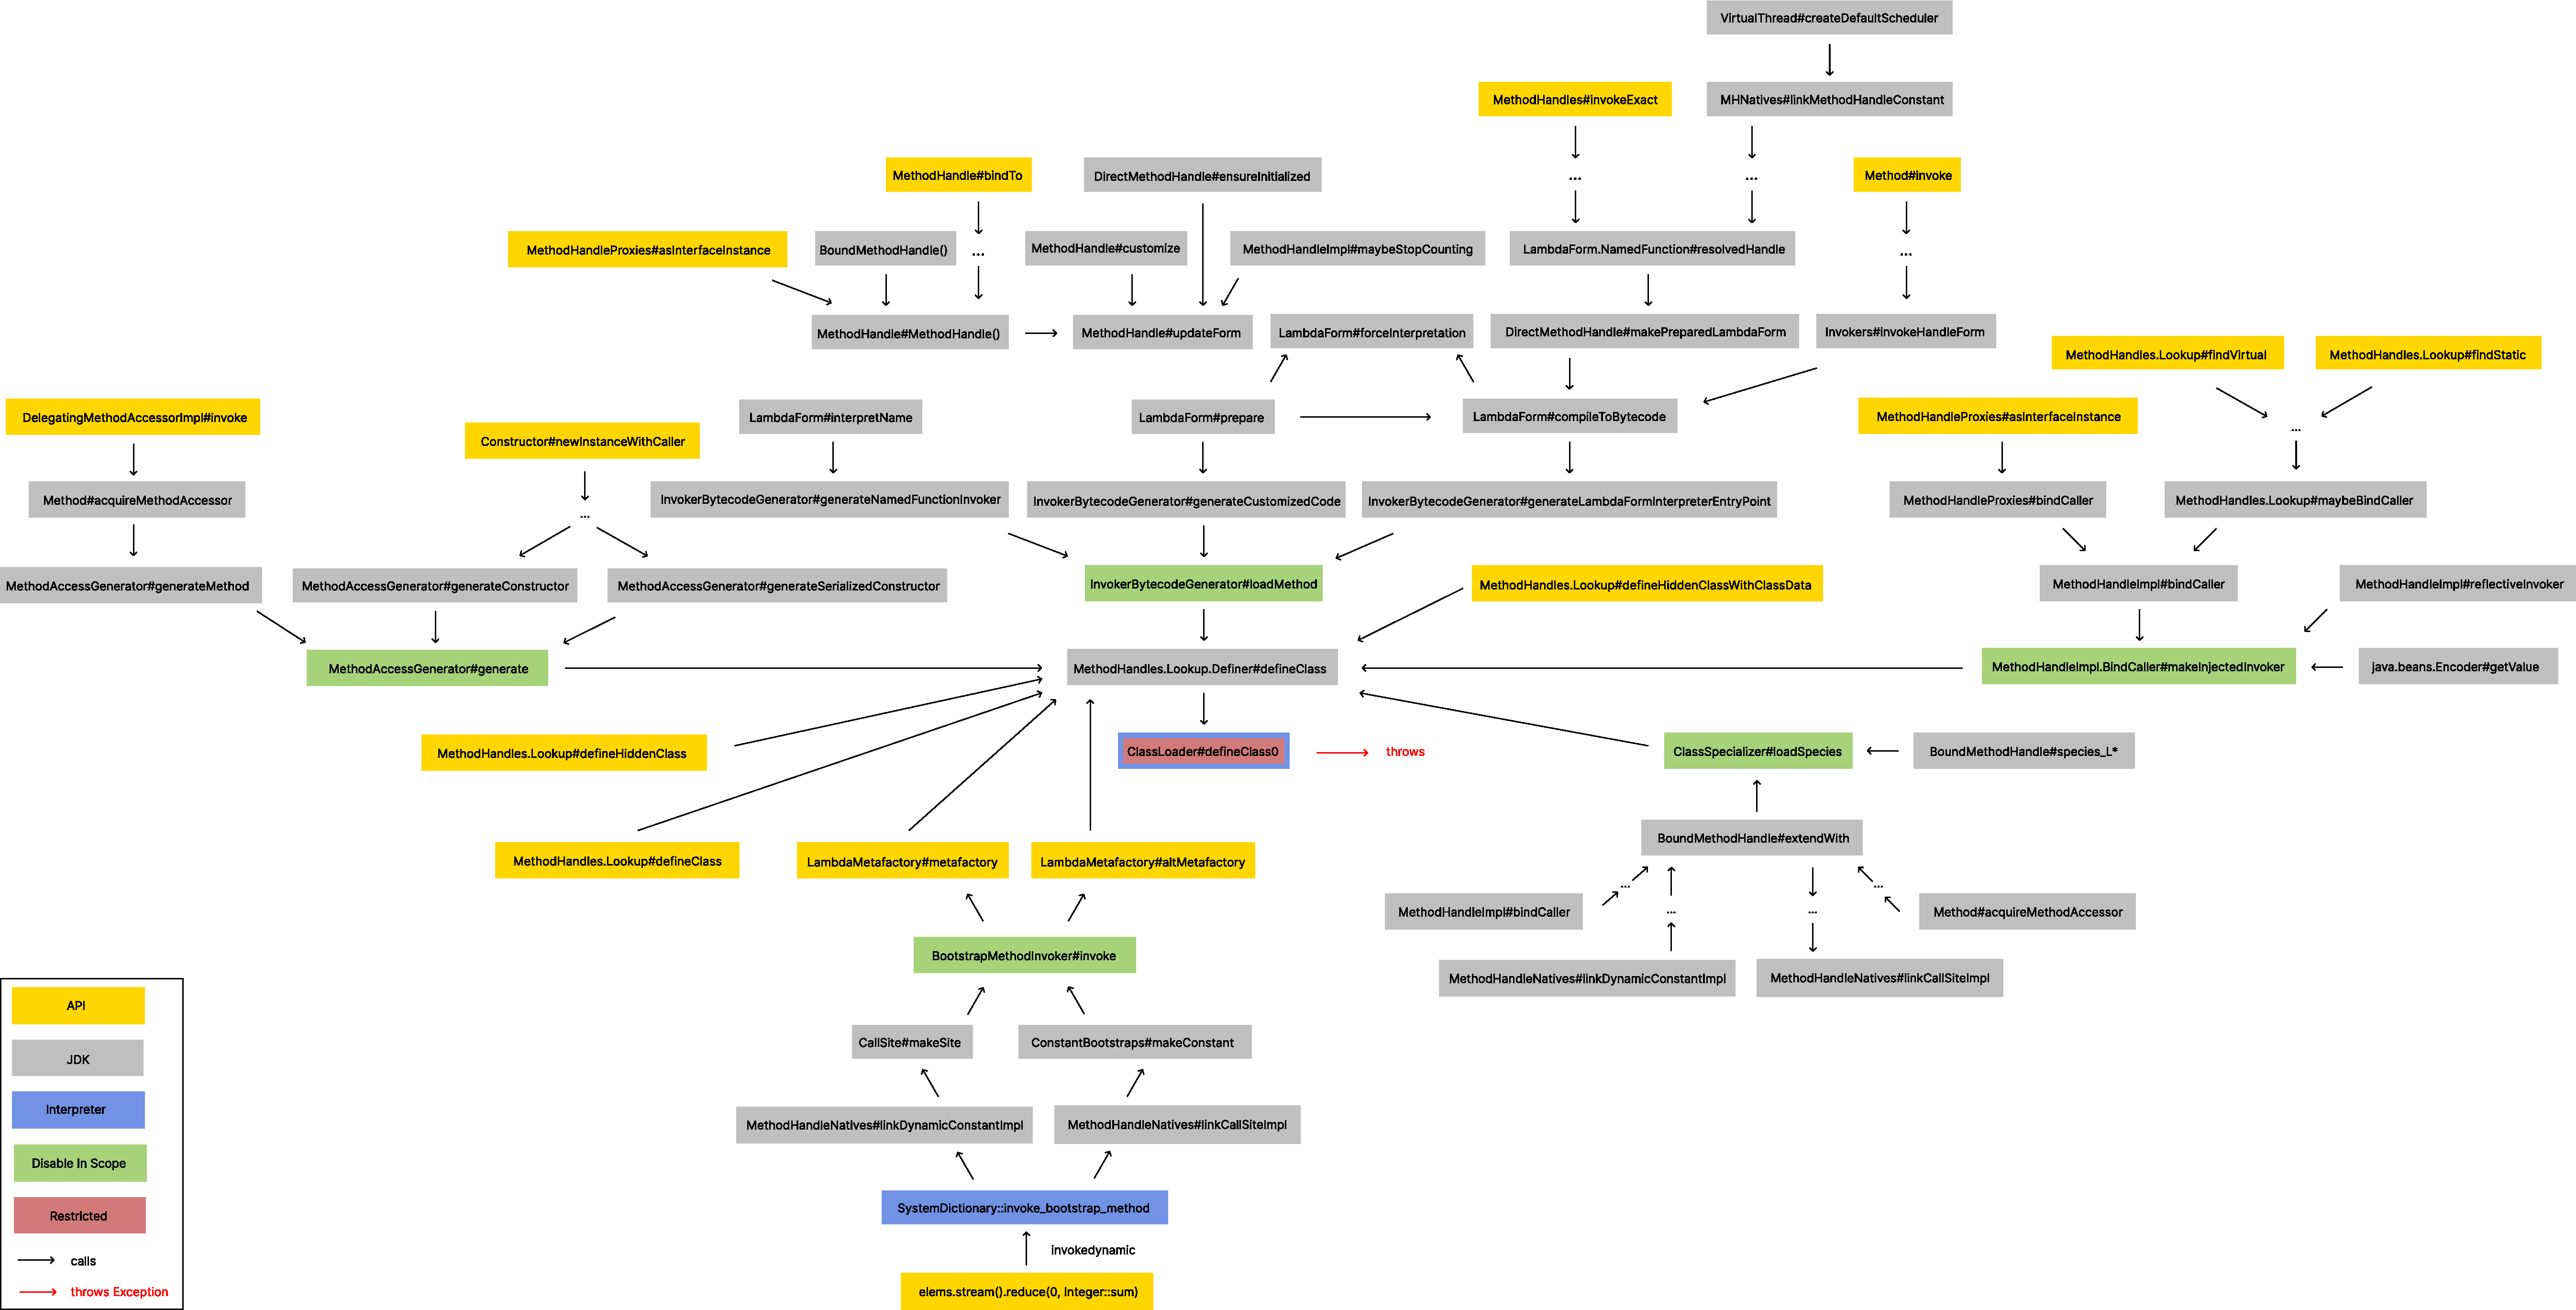
\includegraphics[angle=90,origin=c,scale=0.22]{resources/Group 397.png}
    \caption{Caption}
    \label{fig:define_class_0}
\end{figure}
 % split into files if needed

\end{document}